% Options for packages loaded elsewhere
\PassOptionsToPackage{unicode}{hyperref}
\PassOptionsToPackage{hyphens}{url}
\documentclass[
  ignorenonframetext,
  aspectratio=169,
]{beamer}
\newif\ifbibliography
\usepackage{pgfpages}
\setbeamertemplate{caption}[numbered]
\setbeamertemplate{caption label separator}{: }
\setbeamercolor{caption name}{fg=normal text.fg}
\beamertemplatenavigationsymbolsempty
% remove section numbering
\setbeamertemplate{part page}{
  \centering
  \begin{beamercolorbox}[sep=16pt,center]{part title}
    \usebeamerfont{part title}\insertpart\par
  \end{beamercolorbox}
}
\setbeamertemplate{section page}{
  \centering
  \begin{beamercolorbox}[sep=12pt,center]{section title}
    \usebeamerfont{section title}\insertsection\par
  \end{beamercolorbox}
}
\setbeamertemplate{subsection page}{
  \centering
  \begin{beamercolorbox}[sep=8pt,center]{subsection title}
    \usebeamerfont{subsection title}\insertsubsection\par
  \end{beamercolorbox}
}
% Prevent slide breaks in the middle of a paragraph
\widowpenalties 1 10000
\raggedbottom
\AtBeginPart{
  \frame{\partpage}
}
\AtBeginSection{
  \ifbibliography
  \else
    \frame{\sectionpage}
  \fi
}
\AtBeginSubsection{
  \frame{\subsectionpage}
}
\usepackage{iftex}
\ifPDFTeX
  \usepackage[T1]{fontenc}
  \usepackage[utf8]{inputenc}
  \usepackage{textcomp} % provide euro and other symbols
\else % if luatex or xetex
  \usepackage{unicode-math} % this also loads fontspec
  \defaultfontfeatures{Scale=MatchLowercase}
  \defaultfontfeatures[\rmfamily]{Ligatures=TeX,Scale=1}
\fi
\usepackage{lmodern}
\ifPDFTeX\else
  % xetex/luatex font selection
\fi
% Use upquote if available, for straight quotes in verbatim environments
\IfFileExists{upquote.sty}{\usepackage{upquote}}{}
\IfFileExists{microtype.sty}{% use microtype if available
  \usepackage[]{microtype}
  \UseMicrotypeSet[protrusion]{basicmath} % disable protrusion for tt fonts
}{}
\makeatletter
\@ifundefined{KOMAClassName}{% if non-KOMA class
  \IfFileExists{parskip.sty}{%
    \usepackage{parskip}
  }{% else
    \setlength{\parindent}{0pt}
    \setlength{\parskip}{6pt plus 2pt minus 1pt}}
}{% if KOMA class
  \KOMAoptions{parskip=half}}
\makeatother
\usepackage{longtable,booktabs,array}
\usepackage{caption}
\captionsetup[table]{skip=6pt}
\newcounter{none} % for unnumbered tables
\usepackage{calc} % for calculating minipage widths
\usepackage{caption}
% Make caption package work with longtable
\makeatletter
\def\fnum@table{\tablename~\thetable}
\makeatother
\usepackage{graphicx}
\makeatletter
\newsavebox\pandoc@box
\newcommand*\pandocbounded[1]{% scales image to fit in text height/width
  \sbox\pandoc@box{#1}%
  \Gscale@div\@tempa{\textheight}{\dimexpr\ht\pandoc@box+\dp\pandoc@box\relax}%
  \Gscale@div\@tempb{\linewidth}{\wd\pandoc@box}%
  \ifdim\@tempb\p@<\@tempa\p@\let\@tempa\@tempb\fi% select the smaller of both
  \ifdim\@tempa\p@<\p@\scalebox{\@tempa}{\usebox\pandoc@box}%
  \else\usebox{\pandoc@box}%
  \fi%
}
% Set default figure placement to htbp
\def\fps@figure{htbp}
\makeatother
\setlength{\emergencystretch}{3em} % prevent overfull lines
\providecommand{\tightlist}{%
  \setlength{\itemsep}{0pt}\setlength{\parskip}{0pt}}
% Auto-generated by infrastructure/rendering/_pdf_latex_helpers.py::extract_math_font_preamble.
% Minimal header passed to Pandoc via -H so Beamer slides pick up the same math font
% as the combined-PDF path. Adjust the manuscript's preamble.md to change the font globally.
\usepackage{unicode-math}
\setmathfont{latinmodern-math.otf}

% Manuscript macro/package fallbacks (newcommand -> providecommand).
% Core mathematics
\usepackage{amsmath}
\usepackage{amssymb}
% Document layout
% Tables
\usepackage{booktabs}
% Caption styling (booktabs already loaded above). Small caption font with a
% bold label ("Figure 1", "Table 2") gives the math/figure-heavy layout a
% consistent, journal-like caption rhythm without fighting pandoc-crossref —
% pandoc emits standard \caption{}, and caption/captionsetup only restyle it.
% ── Theorem environments ─────────────────────────────────────────────────
% amsthm is loaded above. The FedGVI<->Friston bridge is stated as a small
% number of theorems/definitions/lemmas/propositions/corollaries; sharing one
% counter (definition/lemma/proposition/corollary all step the `theorem`
% counter) gives a single monotone numbering 1, 2, 3, ... across all kinds, so
% authors can reference them as Theorem 1, Definition 2, Corollary 3 without a
% per-kind counter drifting out of order. Plain style for theorem-like results,
% definition style (upright body) for definitions.
% (algorithm2e intentionally not loaded: this manuscript states results as
% numbered amsthm Theorems/Definitions, not algorithm2e pseudocode.)
% Code listings
\usepackage{listings}
% Typography and formatting
% (siunitx intentionally not loaded: no \SI/\num units appear in this manuscript.)
% Cross-references and citations
% (cleveref and titlesec intentionally not loaded: unavailable in this TeX tree
% and not required. Cross-references resolve through pandoc-crossref's own
% \ref-style names — no \cref appears — and section heading styling falls back
% to the pandoc/LaTeX defaults.)
% ── TeX Live Basic-compatible mono font for code listings ────────────
% Latin Modern Mono is bundled with TeX Live Basic and keeps the manuscript
% renderable on minimal TeX installations. Mathematical Unicode coverage is
% provided separately by Latin Modern Math below, so the code font does not
% need a private JuliaMono installation.
%
% Use the TeX font filename rather than the system-family name: the minimal
% TeX Live fontconfig database may not register the OpenType family even though
% kpsewhich can resolve the bundled files.
% Math font for unicode-math: Latin Modern Math (TeX Live) has full BMP
% coverage including U+2223 (\mid), U+226A/226B (\ll/\gg), and the Greek/
% blackboard letters used in equations. Without an explicit \setmathfont,
% unicode-math falls back to lmroman text font which lacks several glyphs
% and emits "Missing character" warnings on every \mid in math mode.

% Slide layout defaults for warning-clean scientific decks.
\usepackage{etoolbox}
\IfFileExists{xurl.sty}{\usepackage{xurl}}{}
\IfFileExists{seqsplit.sty}{\usepackage{seqsplit}}{\newcommand{\seqsplit}[1]{#1}}
\protected\def\breakseq#1{\seqsplit{#1}}
\protected\def\breaktt#1{\begingroup\ttfamily\seqsplit{#1}\endgroup}
\setlength{\emergencystretch}{6em}
\tolerance=5000
\hbadness=10000
\hfuzz=1pt
\setlength{\tabcolsep}{2pt}
\AtBeginEnvironment{longtable}{\tiny\renewcommand{\arraystretch}{0.86}\setlength{\tabcolsep}{1pt}}
\AtBeginEnvironment{tabular}{\tiny\renewcommand{\arraystretch}{0.86}\setlength{\tabcolsep}{1pt}}
\AtBeginEnvironment{equation}{\tiny}
\AtBeginEnvironment{equation*}{\tiny}
\AtBeginEnvironment{align}{\tiny}
\AtBeginEnvironment{align*}{\tiny}
\AtBeginEnvironment{itemize}{\footnotesize}
\AtBeginEnvironment{enumerate}{\footnotesize}
\AtBeginEnvironment{description}{\footnotesize}
\setbeamerfont{caption}{size=\tiny}
\setbeamerfont{caption name}{size=\tiny}
\setbeamerfont{normal text}{size=\small}
\setbeamerfont{frametitle}{size=\small}
\setbeamerfont{section title}{size=\footnotesize}
\setbeamerfont{subsection title}{size=\footnotesize}
\setbeamertemplate{section page}{%
  \centering
  \begin{beamercolorbox}[sep=12pt,center,wd=\paperwidth]{section title}
    \parbox{0.86\paperwidth}{\centering\usebeamerfont{section title}\insertsection\par}
  \end{beamercolorbox}
}
\setbeamertemplate{subsection page}{%
  \centering
  \begin{beamercolorbox}[sep=8pt,center,wd=\paperwidth]{subsection title}
    \parbox{0.86\paperwidth}{\centering\usebeamerfont{subsection title}\insertsubsection\par}
  \end{beamercolorbox}
}
\setlength{\abovecaptionskip}{2pt}
\setlength{\belowcaptionskip}{0pt}

% Natbib and cross-reference fallbacks — slides don't load natbib
% or cleveref, but combined-PDF manuscript prose may emit these
% commands. The fallback renders citations as a bracketed key list
% and cross-references as detokenized labels so slides don't fail on
% undefined control sequences or raw underscores. \providecommand is
% a no-op if packages load later.
\providecommand{\citep}[1]{[#1]}
\providecommand{\citet}[1]{#1}
\providecommand{\citealp}[1]{#1}
\providecommand{\citeauthor}[1]{#1}
\providecommand{\citeyear}[1]{#1}
\providecommand{\cref}[1]{\texttt{\detokenize{#1}}}
\providecommand{\Cref}[1]{\texttt{\detokenize{#1}}}
\providecommand{\crefrange}[2]{\texttt{\detokenize{#1}}--\texttt{\detokenize{#2}}}
\providecommand{\Crefrange}[2]{\texttt{\detokenize{#1}}--\texttt{\detokenize{#2}}}
\providecommand{\paragraph}[1]{\textbf{#1}\ }

% Opt-in accessible presentation profile.
\setbeamerfont{normal text}{size*={20pt}{24pt}}
\setbeamerfont{frametitle}{size*={28pt}{32pt}}
\setbeamerfont{section title}{size*={28pt}{32pt}}
\setbeamerfont{subsection title}{size*={28pt}{32pt}}
\setbeamerfont{caption}{size*={16pt}{19pt}}
\setbeamerfont{caption name}{size*={16pt}{19pt}}
\setbeamerfont{itemize/enumerate body}{size*={20pt}{24pt}}
\setbeamerfont{itemize/enumerate subbody}{size*={20pt}{24pt}}
\setbeamerfont{itemize/enumerate subsubbody}{size*={20pt}{24pt}}
\setbeamerfont{itemize item}{size*={20pt}{24pt}}
\setbeamerfont{itemize subitem}{size*={20pt}{24pt}}
\setbeamerfont{itemize subsubitem}{size*={20pt}{24pt}}
\setbeamerfont{description body}{size*={20pt}{24pt}}
\setbeamerfont{description item}{size*={20pt}{24pt}}
\setbeamerfont{quote}{size*={20pt}{24pt}}
\setbeamerfont{quotation}{size*={20pt}{24pt}}
\AtBeginEnvironment{longtable}{\fontsize{20pt}{24pt}\selectfont}
\AtBeginEnvironment{tabular}{\fontsize{20pt}{24pt}\selectfont}
\AtBeginEnvironment{equation}{\fontsize{20pt}{24pt}\selectfont}
\AtBeginEnvironment{equation*}{\fontsize{20pt}{24pt}\selectfont}
\AtBeginEnvironment{align}{\fontsize{20pt}{24pt}\selectfont}
\AtBeginEnvironment{align*}{\fontsize{20pt}{24pt}\selectfont}
\AtBeginEnvironment{itemize}{\fontsize{20pt}{24pt}\selectfont}
\AtBeginEnvironment{enumerate}{\fontsize{20pt}{24pt}\selectfont}
\AtBeginEnvironment{description}{\fontsize{20pt}{24pt}\selectfont}
\AtBeginDocument{\usebeamerfont{normal text}}
\newlength{\AFSlideTableWidth}
% The fixed footer reservation is calibrated with the semantic seven-line regular-body budget.
\setbeamertemplate{footline}{%
  \leavevmode\vbox{%
    \hbox{%
      \begin{beamercolorbox}[wd=\paperwidth,ht=16pt,dp=3pt,center]{author in head/foot}%
        \fontsize{16pt}{19pt}\selectfont Untagged PDF derivative \textbar\ \href{../web/index.html}{HTML reader}%
      \end{beamercolorbox}%
    }%
    \vskip6pt%
  }%
}
% Accessible footer reserved height: 25pt.

\newtheorem{proposition}{Proposition}
\newtheorem{hypothesis}{Hypothesis}
\newtheorem{remark}[theorem]{Remark}
\newtheorem{axiom}{Axiom}
\newtheorem{property}{Property}
\usepackage{bookmark}
\IfFileExists{xurl.sty}{\usepackage{xurl}}{} % add URL line breaks if available
\urlstyle{same}
% fallback for those not using the hyperref driver hyperxmp:
\makeatletter
\@ifundefined{xmpquote}{\newcommand{\xmpquote}[1]{#1}}{}
\makeatother
\hypersetup{
  hidelinks,
  pdfcreator={LaTeX via pandoc}}

\author{\texorpdfstring{}{}}
\date{}

\begin{document}

\section{Supplement: extended methods for scoped
generalization}\label{sec:supp-extended}

\begin{frame}{Supplement: extended methods for scoped generalization}
This supplement documents three method extensions that broaden the
toolkit without changing the categorical federated claims of the main
text.
\end{frame}

\begin{frame}{Supplement: extended\ldots{} (part 2)}
Each answers a ``does it generalize?'' question raised by a specific
main-text result and each connects back to it.
\end{frame}

\begin{frame}{Supplement: extended\ldots{} (part 3)}
The additional contamination models, gallery, and onset sweep
stress-test the robustness verdict of sec.~7.5
beyond its single confident-wrong mechanism; the Gaussian divergence
bridge points toward the continuous-state direction of
sec.~8.22;
\end{frame}

\begin{frame}{Supplement: extended\ldots{} (part 4)}
and greedy multi-hypothesis reduction extends the configured BMR sign
control of sec.~7.4 from one pruned state to a
family.
\end{frame}

\begin{frame}{Supplement: extended\ldots{} (part 5)}
Each is tested and isolated; none participates in the headline
robustness verdict, so the main-text claims stand or fall without them.
\end{frame}

\begin{frame}{Continuous-state divergence bridge for Gaussian beliefs}
\protect\phantomsection\label{sec:supp-gaussian}
Every robustness claim in the main text is discrete-categorical,
matching Friston's worked example.
\end{frame}

\begin{frame}[fragile]{Continuous-state divergence\ldots{} (part 2)}
To show the divergence family carries over to the Gaussian beliefs a
continuous-state active-inference extension would use,
\texttt{divergences.py} adds closed forms for 1-D Gaussians: the
Kullback--Leibler divergence
\end{frame}

\begin{frame}{Continuous-state divergence\ldots{} (part 3)}
\begin{equation}\tag{32}\protect\phantomsection\label{eq:gaussian-kl}{
\begin{aligned}
&\mathrm{KL}\!\big(
  \mathcal N(\mu_q,\sigma_q^2)\,\|\,\mathcal N(\mu_p,\sigma_p^2)\big)\\
&\quad = \tfrac12\!\left[
\begin{aligned}
&\tfrac{\sigma_q^2}{\sigma_p^2}
 + \tfrac{(\mu_p-\mu_q)^2}{\sigma_p^2}\\
&\quad - 1 + \log\tfrac{\sigma_p^2}{\sigma_q^2}
\end{aligned}
\right].
\end{aligned}
}\end{equation}
\end{frame}

\begin{frame}{Continuous-state divergence\ldots{} (part 4)}
and the \(\alpha\)-Rényi divergence with interpolated variance
\(\sigma_\alpha^2 = \alpha\sigma_p^2 + (1-\alpha)\sigma_q^2\),
\end{frame}

\begin{frame}{Continuous-state divergence\ldots{} (part 5)}
\begin{equation}\tag{33}\protect\phantomsection\label{eq:gaussian-renyi}{
\begin{aligned}
&D_\alpha\!\big(\mathcal N_q\,\|\,\mathcal N_p\big)\\
&\quad = \frac{\alpha(\mu_q-\mu_p)^2}{2\sigma_\alpha^2}\\
&\qquad - \frac{1}{2(\alpha-1)}
\log\frac{\sigma_\alpha^2}
{\sigma_q^{2(1-\alpha)}\sigma_p^{2\alpha}}.
\end{aligned}
}\end{equation}
\end{frame}

\begin{frame}{Continuous-state divergence\ldots{} (part 6)}
As in the categorical case (eq.~6 and Lemma
3), eq.~33 recovers
eq.~32 in the \(\alpha\to1\) limit, and the closed
form is returned exactly inside a small band around one. These functions
are \textbf{out of scope} for the federated experiments ---
\end{frame}

\begin{frame}{Continuous-state divergence\ldots{} (part 7)}
they are wired into no aggregation rule or sweep --- and exist purely as
the explicitly-scoped bridge toward continuous active inference.
\end{frame}

\begin{frame}[fragile]{Additional contamination models for the
robustness surface}
\protect\phantomsection\label{sec:supp-contamination}
\texttt{contamination.py} extends the confident-wrong, label-noise, and
uniform models with two mechanisms that probe different attack surfaces,
both honoring the identity anchor (rate zero returns the belief
unchanged):
\end{frame}

\begin{frame}{Additional contamination\ldots{} (part 2)}
\textbf{Byzantine targeted.} A \emph{multiplicative} log-odds tilt
toward an adversary-chosen state,
\(s' \propto s\cdot\exp(\text{rate}\cdot\text{tilt}\cdot e_{\text{target}})\).
Unlike the additive convex mixes,
\end{frame}

\begin{frame}{Additional contamination\ldots{} (part 3)}
the corruption compounds with the belief's own shape, so the non-target
states keep their relative order --- the canonical targeted poisoning of
a product-of-experts pool.
\end{frame}

\begin{frame}{Additional contamination\ldots{} (part 4)}
\textbf{Drift.} A \emph{slowly-moving} bias grows linearly across
communication rounds via a phase
\(\phi = \text{round}/(\text{rounds}-1)\), so the first round is clean
and the bias creeps in. This is the stealthy sentinel whose
miscalibration only becomes confident late, defeating any one-shot
screen.
\end{frame}

\begin{frame}{Additional contamination\ldots{} (part 5)}
Both are exercised in the contamination tests; the headline sweep
continues to use the confident-wrong model so the verdict is comparable
to the main text.
\end{frame}

\begin{frame}{Contamination gallery by corruption mechanism}
\protect\phantomsection\label{sec:supp-gallery}
To check the robust-beats-naive result is not an artifact of the single
confident-wrong mechanism --- and not of a single lucky seed ---
\end{frame}

\begin{frame}[fragile]{Contamination gallery by\ldots{} (part 2)}
the \texttt{run\_contamination\_gallery} function in the
\texttt{experiments} module re-runs the paired comparison (\(n = 24\)
trials across 64 independent seeds, contamination strength 0.60) under
every model.
\end{frame}

\begin{frame}{Contamination gallery by\ldots{} (part 3)}
For each mechanism it selects one robust method by pooled mean consensus
accuracy \textbf{for descriptive gallery display only}, then reports
that displayed member's robust-minus-naive difference, 95\% seed
bootstrap interval, and \emph{win fraction} --- the fraction of seeds in
which the displayed member beats naive.
\end{frame}

\begin{frame}{Contamination gallery by\ldots{} (part 4)}
This is not the selection-free inferential surface; the main-text
all-method review grid in sec.~7.5.1 serves that
role.
\end{frame}

\begin{frame}{Contamination gallery by\ldots{} (part 5)}
% template-accessible-table-inset
\begingroup
\setlength{\AFSlideTableWidth}{\textwidth}%
\setlength{\LTleft}{\fill}%
\setlength{\LTright}{\fill}%
\begin{longtable}[]{@{}
  >{\raggedright\arraybackslash}p{(\AFSlideTableWidth - 6\tabcolsep) * \real{0.2750}}
  >{\raggedright\arraybackslash}p{(\AFSlideTableWidth - 6\tabcolsep) * \real{0.2500}}
  >{\raggedright\arraybackslash}p{(\AFSlideTableWidth - 6\tabcolsep) * \real{0.1727}}
  >{\raggedright\arraybackslash}p{(\AFSlideTableWidth - 6\tabcolsep) * \real{0.3023}}@{}}
\label{tbl:contamination-gallery}\tabularnewline
\toprule\noalign{}
\begin{minipage}[b]{\linewidth}\raggedright
Mechanism
\end{minipage} & \begin{minipage}[b]{\linewidth}\raggedright
Class
\end{minipage} & \begin{minipage}[b]{\linewidth}\raggedright
Naive mean
\end{minipage} & \begin{minipage}[b]{\linewidth}\raggedright
Display robust mean (preset)
\end{minipage} \\
\midrule\noalign{}
\endfirsthead
\toprule\noalign{}
\begin{minipage}[b]{\linewidth}\raggedright
Mechanism
\end{minipage} & \begin{minipage}[b]{\linewidth}\raggedright
Class
\end{minipage} & \begin{minipage}[b]{\linewidth}\raggedright
Naive mean
\end{minipage} & \begin{minipage}[b]{\linewidth}\raggedright
Display robust mean (preset)
\end{minipage} \\
\midrule\noalign{}
\endhead
byzantine & directional & 0.6306 & 0.6599 (beta) \\
confident wrong & directional & 0.9836 & 0.9878 (AR) \\
\bottomrule\noalign{}
\end{longtable}
\endgroup
\end{frame}

\begin{frame}{Contamination gallery by\ldots{} (part 6)}
% template-accessible-table-inset
\begingroup
\setlength{\AFSlideTableWidth}{\textwidth}%
\setlength{\LTleft}{\fill}%
\setlength{\LTright}{\fill}%
\begin{longtable}[]{@{}
  >{\raggedright\arraybackslash}p{(\AFSlideTableWidth - 8\tabcolsep) * \real{0.2821}}
  >{\raggedright\arraybackslash}p{(\AFSlideTableWidth - 8\tabcolsep) * \real{0.1538}}
  >{\raggedright\arraybackslash}p{(\AFSlideTableWidth - 8\tabcolsep) * \real{0.1795}}
  >{\raggedright\arraybackslash}p{(\AFSlideTableWidth - 8\tabcolsep) * \real{0.1795}}
  >{\raggedright\arraybackslash}p{(\AFSlideTableWidth - 8\tabcolsep) * \real{0.2051}}@{}}
\label{tbl:contamination-gallery-contrast}\tabularnewline
\toprule\noalign{}
\begin{minipage}[b]{\linewidth}\raggedright
Mechanism
\end{minipage} & \begin{minipage}[b]{\linewidth}\raggedright
Mean robust - naive
\end{minipage} & \begin{minipage}[b]{\linewidth}\raggedright
95\% CI
\end{minipage} & \begin{minipage}[b]{\linewidth}\raggedright
Win fraction
\end{minipage} & \begin{minipage}[b]{\linewidth}\raggedright
Reliable
\end{minipage} \\
\midrule\noalign{}
\endfirsthead
\toprule\noalign{}
\begin{minipage}[b]{\linewidth}\raggedright
Mechanism
\end{minipage} & \begin{minipage}[b]{\linewidth}\raggedright
Mean robust - naive
\end{minipage} & \begin{minipage}[b]{\linewidth}\raggedright
95\% CI
\end{minipage} & \begin{minipage}[b]{\linewidth}\raggedright
Win fraction
\end{minipage} & \begin{minipage}[b]{\linewidth}\raggedright
Reliable
\end{minipage} \\
\midrule\noalign{}
\endhead
byzantine & 0.0293 & {[}0.0124, 0.0472{]} & 0.62 & No \\
\bottomrule\noalign{}
\end{longtable}
\endgroup
\end{frame}

\begin{frame}{Contamination gallery by\ldots{} (part 7)}
The paired contamination summaries
tbls.~14, 15
form one descriptive sensitivity screen, deliberately narrower than
``robust always wins.'' The pooled display member has a positive
all-seed and interval pattern under confident wrong, drift ---
\end{frame}

\begin{frame}{Contamination gallery by\ldots{} (part 8)}
the \emph{additive} directional attacks.

The full set of directional mechanisms is confident wrong, byzantine,
drift; the \textbf{byzantine} attack is directional too, but its
\emph{multiplicative} log-odds tilt escalates faster:
\end{frame}

\begin{frame}{Contamination gallery by\ldots{} (part 9)}
at this strength it sits near a veto cliff where the naive pool is
already badly degraded and the displayed robust advantage does not hold
across seeds (its win fraction is well below the 0.95 display bar), so
it does not clear the descriptive reliability screen.
\end{frame}

\begin{frame}{Contamination gallery by\ldots{} (part 10)}
The paired mean-difference interval is reported separately in
tbl.~15.
\end{frame}

\begin{frame}{Contamination gallery by\ldots{} (part 11)}
The \textbf{entropy} attacks (label noise, uniform) raise entropy or
inject noise without a fixed wrong target, so the product-of-experts is
not pulled off the truth and there is nothing to beat --- the robust
members stay close rather than winning (naive undegraded by entropy
attacks: Yes).
\end{frame}

\begin{frame}{Contamination gallery by\ldots{} (part 12)}
fig.~22 draws all mechanisms with their win
fractions. This is the honest scope of this configured gallery: its
displayed members separate from naive under the declared \emph{sustained
additive} directional contamination, stay close under the declared
entropy attacks,
\end{frame}

\begin{frame}{Contamination gallery by\ldots{} (part 13)}
and lose the displayed advantage against the tested multiplicative
adversary near the veto regime.
\end{frame}

\begin{frame}{Contamination gallery by\ldots{} (part 14)}
These finite cells do not establish the same ordering for every attack
strength or world, and they do not turn a pooled display selection into
selection-free inference.
\end{frame}

\begin{frame}{Contamination gallery by\ldots{} (part 15)}
\begin{figure}
\centering
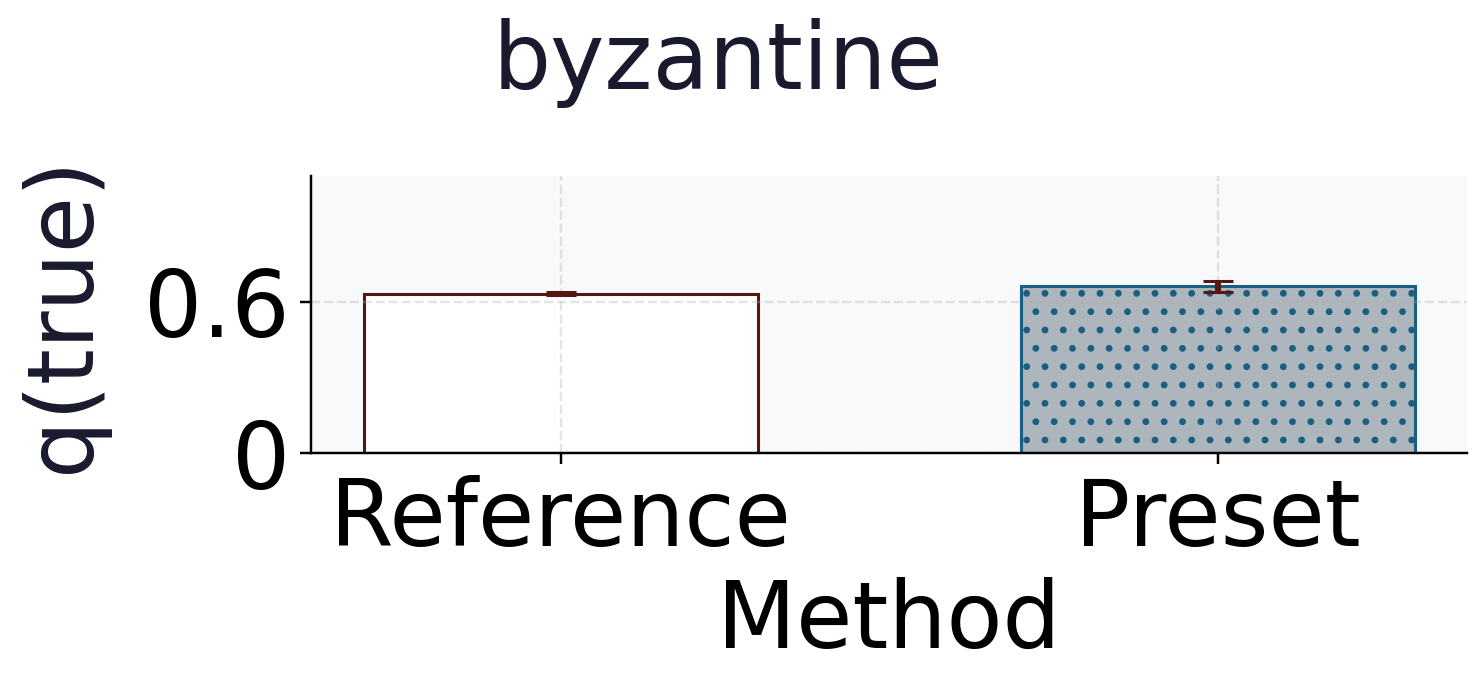
\includegraphics[keepaspectratio,width=0.98\linewidth,height=0.8\textheight,alt={byzantine: reference versus selected server preset, its own source interval, and the declared filled or dotted display flag.}]{../figures/contamination_gallery.slide-mechanism-1.png}
\refstepcounter{figure}\label{fig:contamination-gallery-slide-panel-1}
\end{figure}
\end{frame}

\begin{frame}{Contamination gallery by\ldots{} (part 16)}
\begin{figure}
\centering
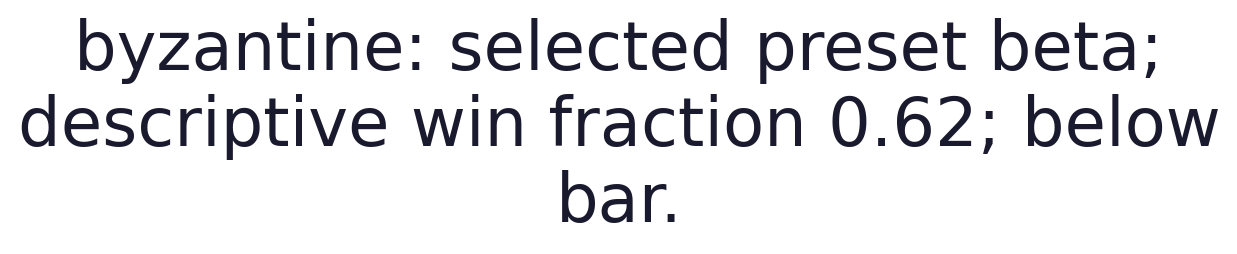
\includegraphics[keepaspectratio,width=0.98\linewidth,height=0.8\textheight,alt={byzantine: selected preset beta; descriptive win fraction 0.62; below bar.}]{../figures/contamination_gallery.slide-mechanism-1-selection.png}
\refstepcounter{figure}\label{fig:contamination-gallery-slide-panel-2}
\end{figure}
\end{frame}

\begin{frame}{Contamination gallery by\ldots{} (part 17)}
\begin{figure}
\centering
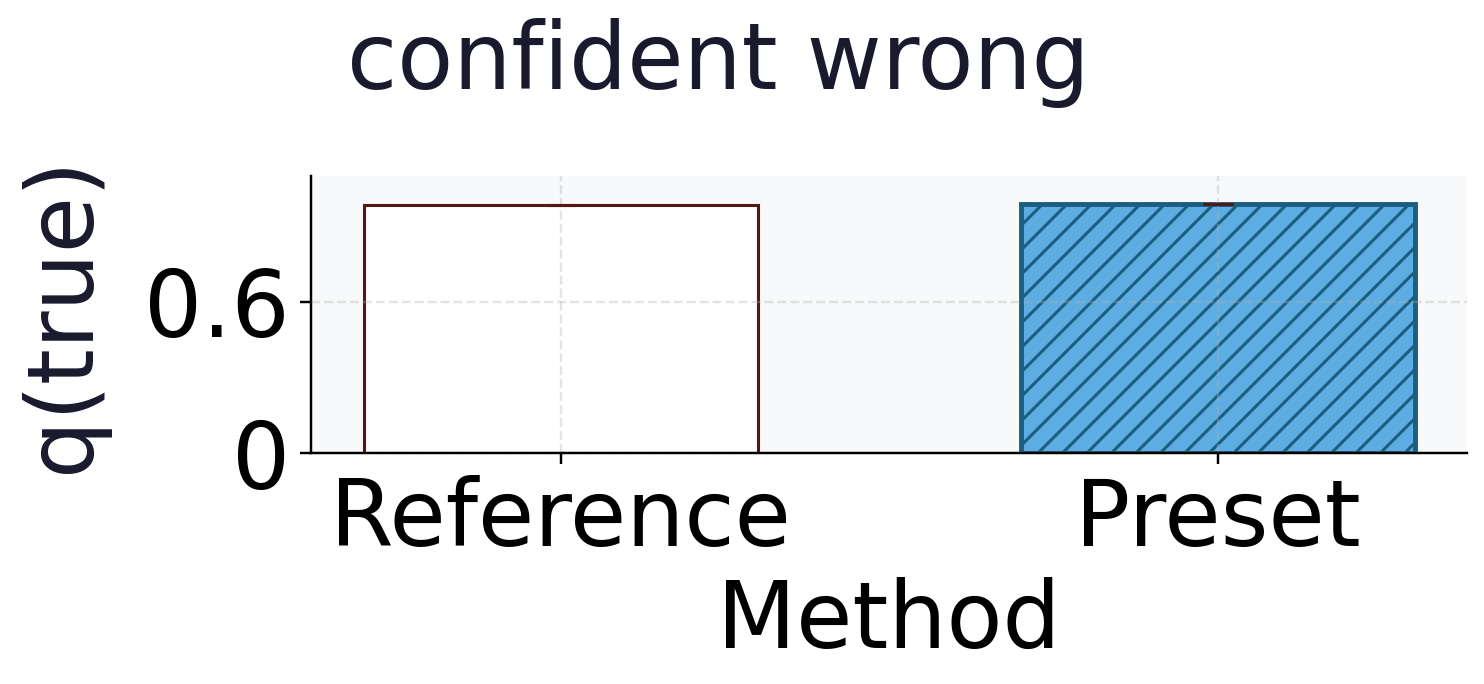
\includegraphics[keepaspectratio,width=0.98\linewidth,height=0.8\textheight,alt={confident\_wrong: reference versus selected server preset, its own source interval, and the declared filled or dotted display flag.}]{../figures/contamination_gallery.slide-mechanism-2.png}
\refstepcounter{figure}\label{fig:contamination-gallery-slide-panel-3}
\end{figure}
\end{frame}

\begin{frame}{Contamination gallery by\ldots{} (part 18)}
\begin{figure}
\centering
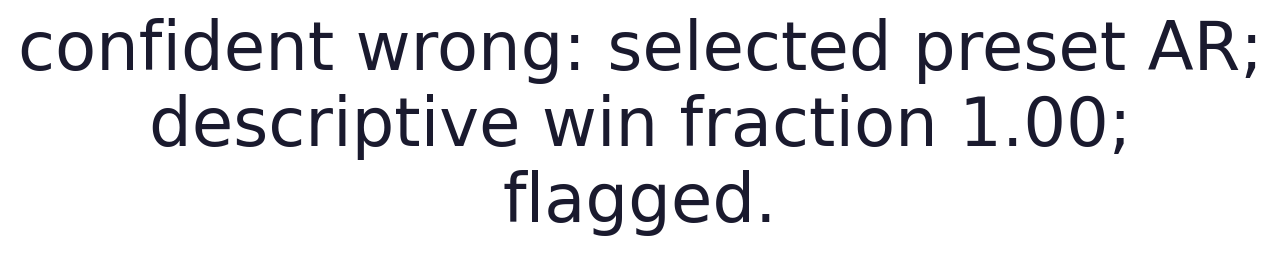
\includegraphics[keepaspectratio,width=0.98\linewidth,height=0.8\textheight,alt={confident wrong: selected preset AR; descriptive win fraction 1.00; flagged.}]{../figures/contamination_gallery.slide-mechanism-2-selection.png}
\refstepcounter{figure}\label{fig:contamination-gallery-slide-panel-4}
\end{figure}
\end{frame}

\begin{frame}{Contamination gallery by\ldots{} (part 19)}
\begin{figure}
\centering
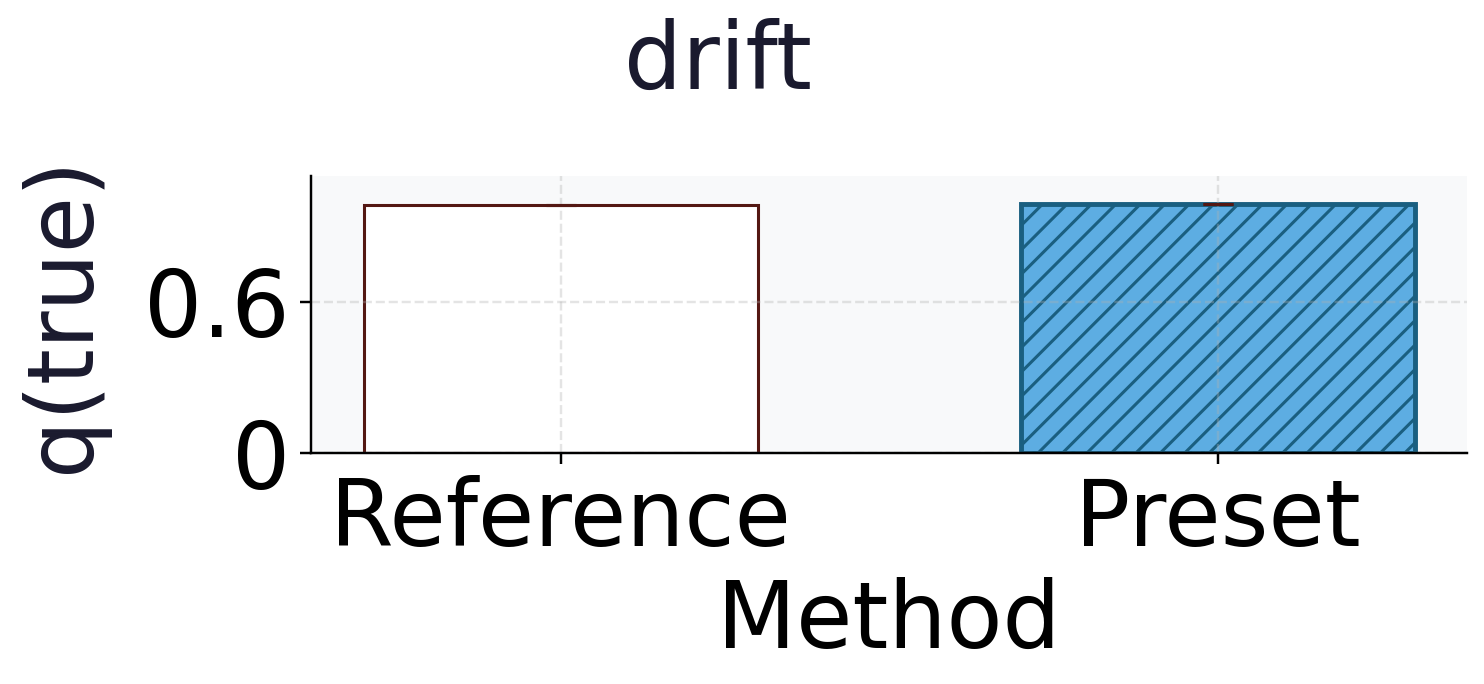
\includegraphics[keepaspectratio,width=0.98\linewidth,height=0.8\textheight,alt={drift: reference versus selected server preset, its own source interval, and the declared filled or dotted display flag.}]{../figures/contamination_gallery.slide-mechanism-3.png}
\refstepcounter{figure}\label{fig:contamination-gallery-slide-panel-5}
\end{figure}
\end{frame}

\begin{frame}{Contamination gallery by\ldots{} (part 20)}
\begin{figure}
\centering
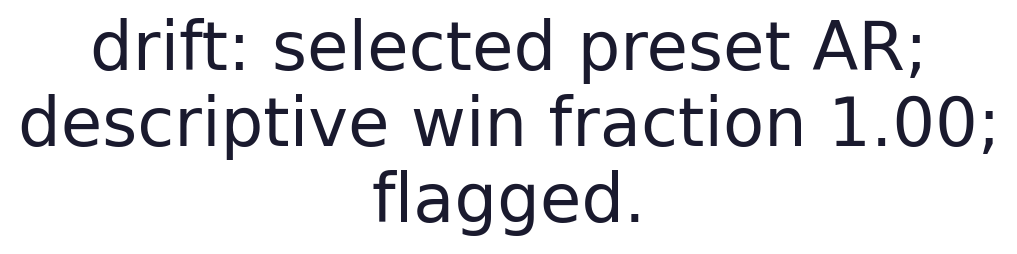
\includegraphics[keepaspectratio,width=0.98\linewidth,height=0.8\textheight,alt={drift: selected preset AR; descriptive win fraction 1.00; flagged.}]{../figures/contamination_gallery.slide-mechanism-3-selection.png}
\refstepcounter{figure}\label{fig:contamination-gallery-slide-panel-6}
\end{figure}
\end{frame}

\begin{frame}{Contamination gallery by\ldots{} (part 21)}
\begin{figure}
\centering
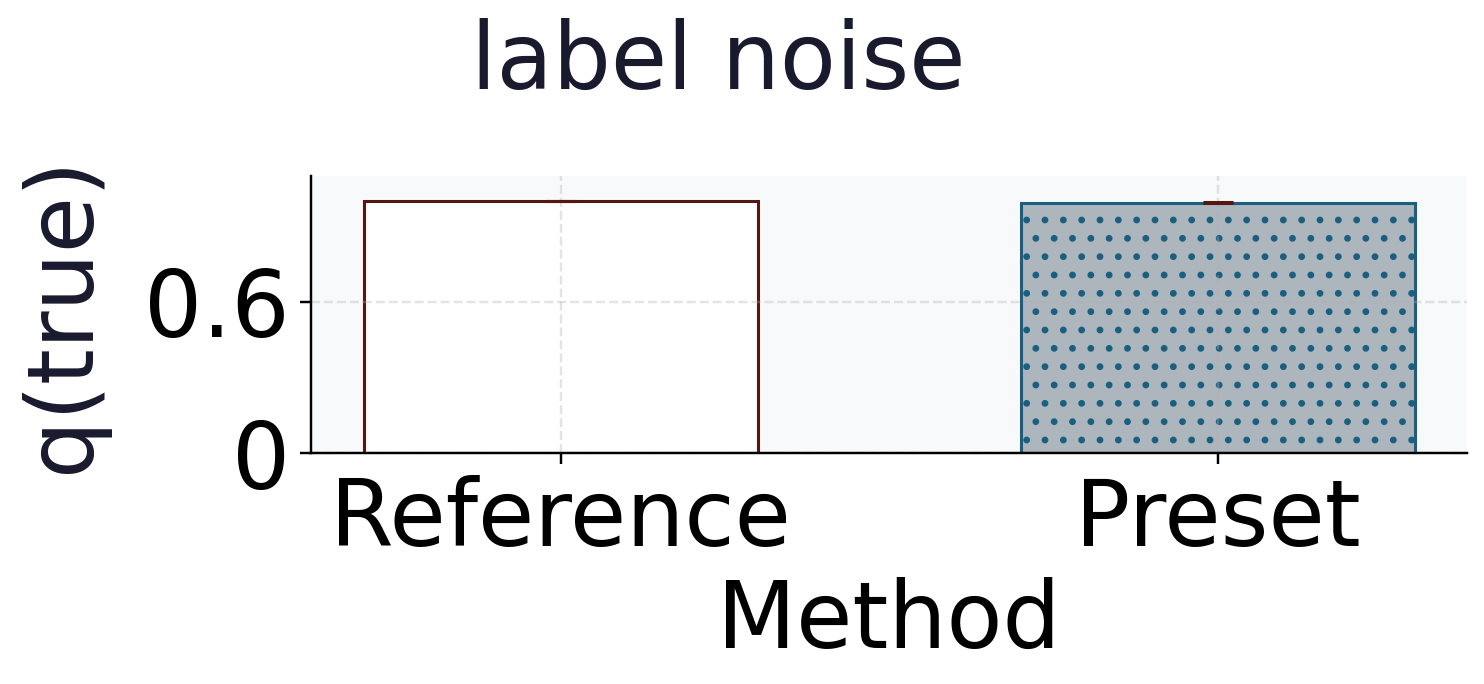
\includegraphics[keepaspectratio,width=0.98\linewidth,height=0.8\textheight,alt={label\_noise: reference versus selected server preset, its own source interval, and the declared filled or dotted display flag.}]{../figures/contamination_gallery.slide-mechanism-4.png}
\refstepcounter{figure}\label{fig:contamination-gallery-slide-panel-7}
\end{figure}
\end{frame}

\begin{frame}{Contamination gallery by\ldots{} (part 22)}
\begin{figure}
\centering
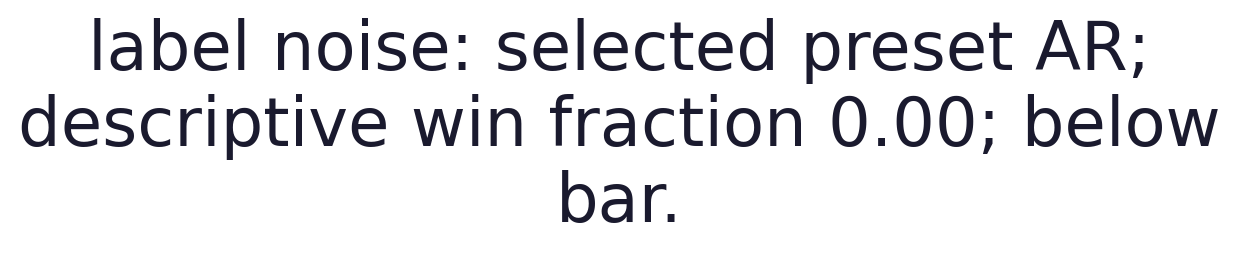
\includegraphics[keepaspectratio,width=0.98\linewidth,height=0.8\textheight,alt={label noise: selected preset AR; descriptive win fraction 0.00; below bar.}]{../figures/contamination_gallery.slide-mechanism-4-selection.png}
\refstepcounter{figure}\label{fig:contamination-gallery-slide-panel-8}
\end{figure}
\end{frame}

\begin{frame}{Contamination gallery by\ldots{} (part 23)}
\begin{figure}
\centering
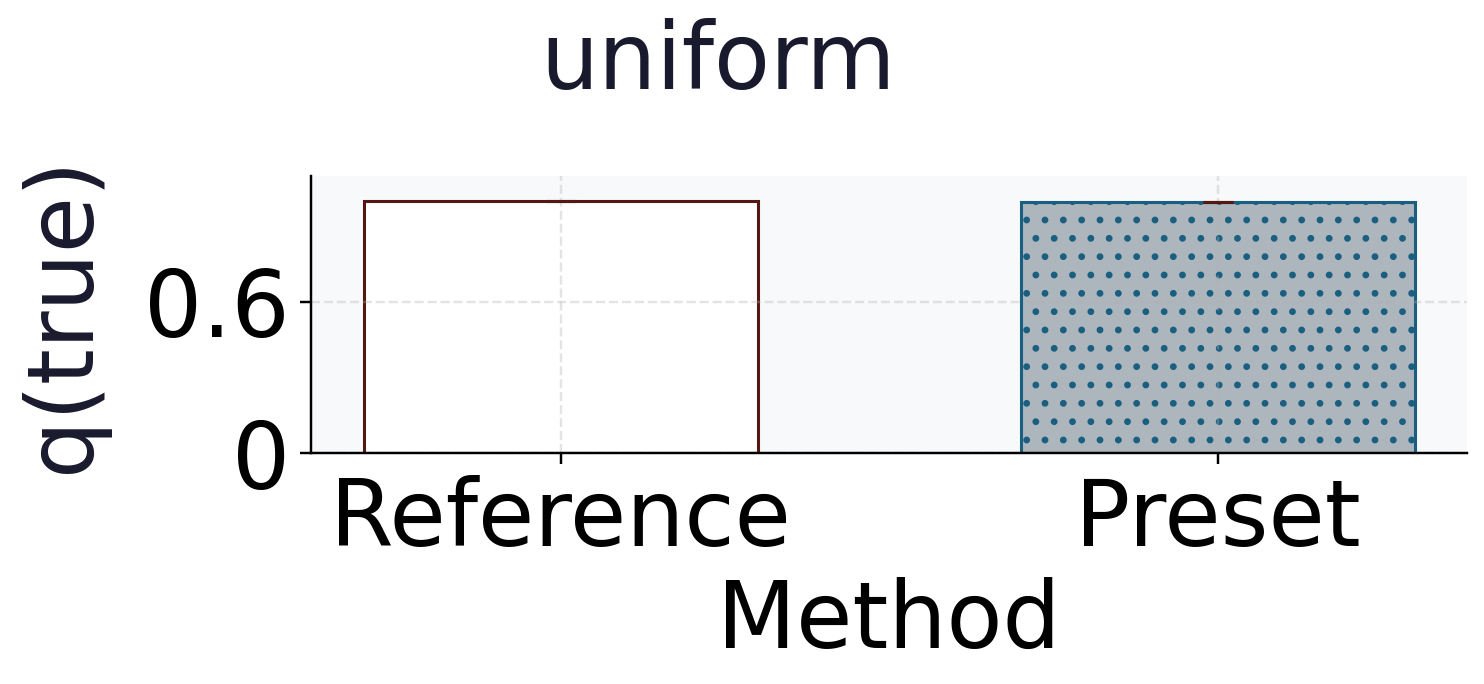
\includegraphics[keepaspectratio,width=0.98\linewidth,height=0.8\textheight,alt={uniform: reference versus selected server preset, its own source interval, and the declared filled or dotted display flag.}]{../figures/contamination_gallery.slide-mechanism-5.png}
\refstepcounter{figure}\label{fig:contamination-gallery-slide-panel-9}
\end{figure}
\end{frame}

\begin{frame}{Contamination gallery by\ldots{} (part 24)}
\begin{figure}
\centering
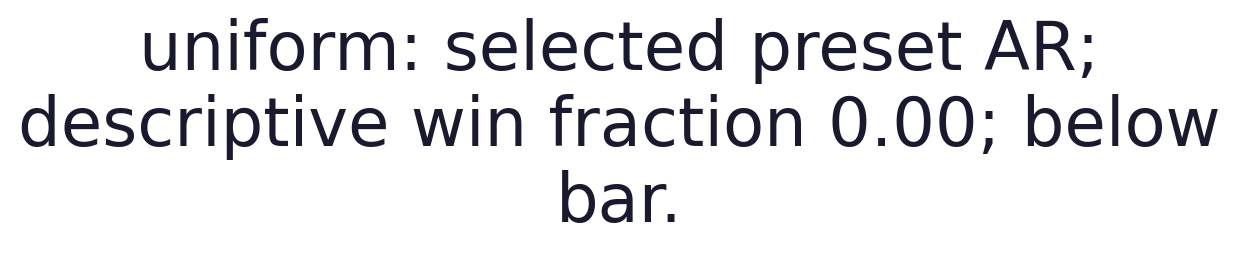
\includegraphics[keepaspectratio,width=0.98\linewidth,height=0.8\textheight,alt={uniform: selected preset AR; descriptive win fraction 0.00; below bar.}]{../figures/contamination_gallery.slide-mechanism-5-selection.png}
\refstepcounter{figure}\label{fig:contamination-gallery-slide-panel-10}
\end{figure}
\end{frame}

\begin{frame}{Contamination gallery by\ldots{} (part 25)}
\begin{figure}
\centering
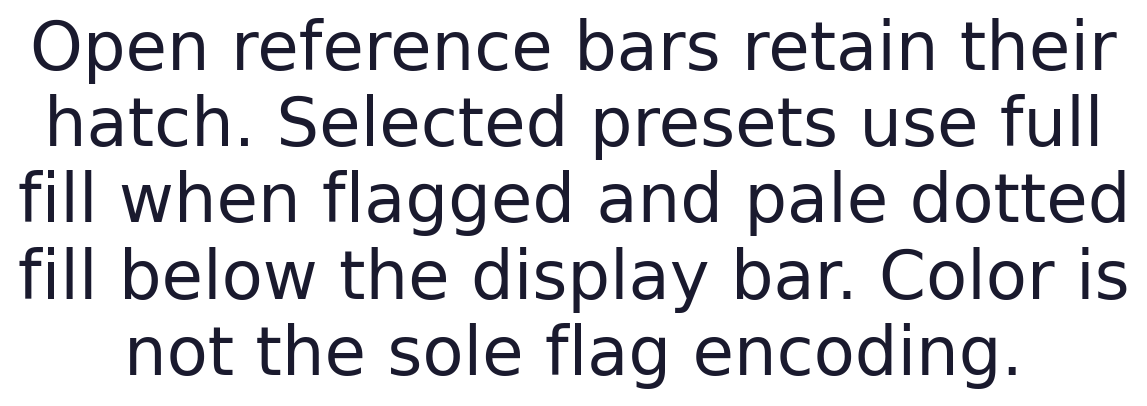
\includegraphics[keepaspectratio,width=0.98\linewidth,height=0.8\textheight,alt={Open reference bars retain their hatch. Selected presets use full fill when flagged and pale dotted fill below the display bar. Color is not the sole flag encoding.}]{../figures/contamination_gallery.slide-key.png}
\refstepcounter{figure}\label{fig:contamination-gallery-slide-panel-11}
\end{figure}
\end{frame}

\begin{frame}{Contamination gallery by\ldots{} (part 26)}
\begin{figure}
\centering
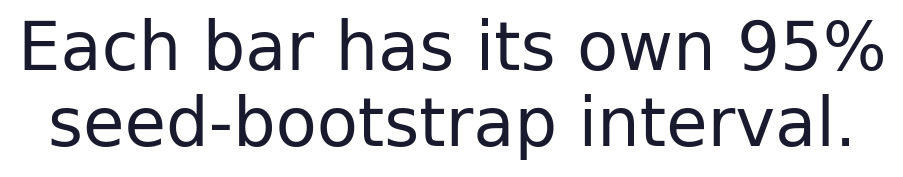
\includegraphics[keepaspectratio,width=0.98\linewidth,height=0.8\textheight,alt={Each bar has its own 95\% seed-bootstrap interval.}]{../figures/contamination_gallery.slide-uncertainty.png}
\refstepcounter{figure}\label{fig:contamination-gallery-slide-panel-12}
\end{figure}
\end{frame}

\begin{frame}{Contamination gallery by\ldots{} (part 27)}
\begin{figure}
\centering
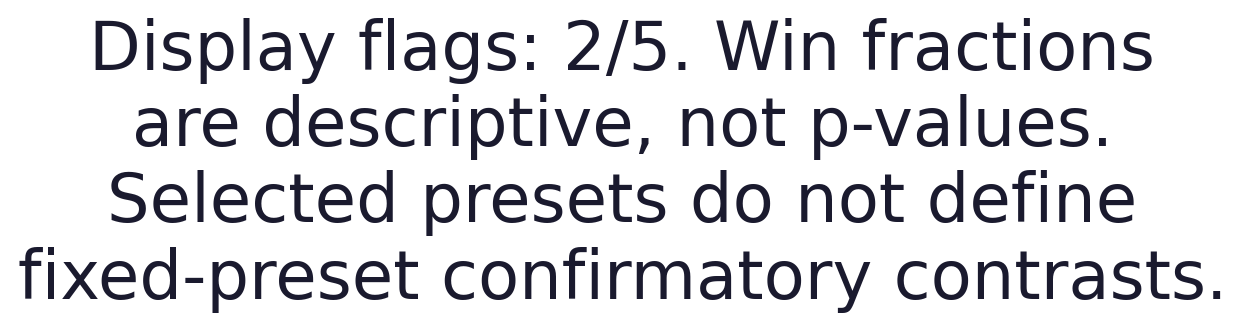
\includegraphics[keepaspectratio,width=0.98\linewidth,height=0.8\textheight,alt={Display flags: 2/5. Win fractions are descriptive, not p-values. Selected presets do not define fixed-preset confirmatory contrasts.}]{../figures/contamination_gallery.slide-scope.png}
\refstepcounter{figure}\label{fig:contamination-gallery-slide-panel-13}
\end{figure}
\end{frame}

\begin{frame}[fragile]{Robustness onset by corruption mechanism}
\protect\phantomsection\label{sec:supp-onset}
The gallery fixes one contamination strength;
\texttt{experiments.run\_robustness\_onset} maps the \emph{rate
dependence} (\(n = 24\) trials \texorpdfstring{\ensuremath{\times}}{x} 64 seeds per rate).
\end{frame}

\begin{frame}{Robustness onset by\ldots{} (part 2)}
For each directional mechanism it reports the \textbf{descriptive onset
rate} --- the smallest rate at which the pooled-selected display
member's win fraction reaches 0.95 ---
\end{frame}

\begin{frame}{Robustness onset by\ldots{} (part 3)}
and that member's versus naive accuracy at the worst (highest) swept
rate. These display summaries are not selection-free inference;

the main-text all-method review grid in
sec.~7.5.1 is the inferential surface:
\end{frame}

\begin{frame}{Robustness onset by\ldots{} (part 4)}
% template-accessible-table-inset
\begingroup
\setlength{\AFSlideTableWidth}{\textwidth}%
\setlength{\LTleft}{\fill}%
\setlength{\LTright}{\fill}%
\begin{longtable}[]{@{}
  >{\raggedright\arraybackslash}p{(\AFSlideTableWidth - 8\tabcolsep) * \real{0.2821}}
  >{\raggedright\arraybackslash}p{(\AFSlideTableWidth - 8\tabcolsep) * \real{0.1436}}
  >{\raggedright\arraybackslash}p{(\AFSlideTableWidth - 8\tabcolsep) * \real{0.1795}}
  >{\raggedright\arraybackslash}p{(\AFSlideTableWidth - 8\tabcolsep) * \real{0.1795}}
  >{\raggedright\arraybackslash}p{(\AFSlideTableWidth - 8\tabcolsep) * \real{0.2154}}@{}}
\label{tbl:robustness-onset}\tabularnewline
\toprule\noalign{}
\begin{minipage}[b]{\linewidth}\raggedright
Mechanism
\end{minipage} & \begin{minipage}[b]{\linewidth}\raggedright
Onset rate
\end{minipage} & \begin{minipage}[b]{\linewidth}\raggedright
Naive @ worst
\end{minipage} & \begin{minipage}[b]{\linewidth}\raggedright
Robust @ worst
\end{minipage} & \begin{minipage}[b]{\linewidth}\raggedright
Robust method @ worst
\end{minipage} \\
\midrule\noalign{}
\endfirsthead
\toprule\noalign{}
\begin{minipage}[b]{\linewidth}\raggedright
Mechanism
\end{minipage} & \begin{minipage}[b]{\linewidth}\raggedright
Onset rate
\end{minipage} & \begin{minipage}[b]{\linewidth}\raggedright
Naive @ worst
\end{minipage} & \begin{minipage}[b]{\linewidth}\raggedright
Robust @ worst
\end{minipage} & \begin{minipage}[b]{\linewidth}\raggedright
Robust method @ worst
\end{minipage} \\
\midrule\noalign{}
\endhead
byzantine & 0.4 & 0.0165 & 0.0000 & beta \\
confident wrong & 0.6 & 0.6676 & 0.7772 & beta \\
\bottomrule\noalign{}
\end{longtable}
\endgroup
\end{frame}

\begin{frame}{Robustness onset by\ldots{} (part 5)}
The mechanism-specific onset thresholds are collected in
tbl.~16.
\end{frame}

\begin{frame}{Robustness onset by\ldots{} (part 6)}
The rate dependence sharpens the gallery's snapshot, and
fig.~23 draws it. The additive confident-wrong
and drift attacks degrade the naive pool gradually; past their onset
rate the robust member stays above it through to the worst rate.
\end{frame}

\begin{frame}{Robustness onset by\ldots{} (part 7)}
The multiplicative byzantine attack is qualitatively different: it opens
an \emph{early} robustness window --- robust overtakes at a lower onset
rate --- but then escalates to the veto cliff where naive and robust
both collapse, so its worst-rate accuracy is near zero for both.
\end{frame}

\begin{frame}{Robustness onset by\ldots{} (part 8)}
This is the rate-resolved bounded interpretation: the displayed contrast
is sustained against the two additive directional mechanisms and only
transient against the multiplicative mechanism.
\end{frame}

\begin{frame}{Robustness onset by\ldots{} (part 9)}
\begin{figure}
\centering
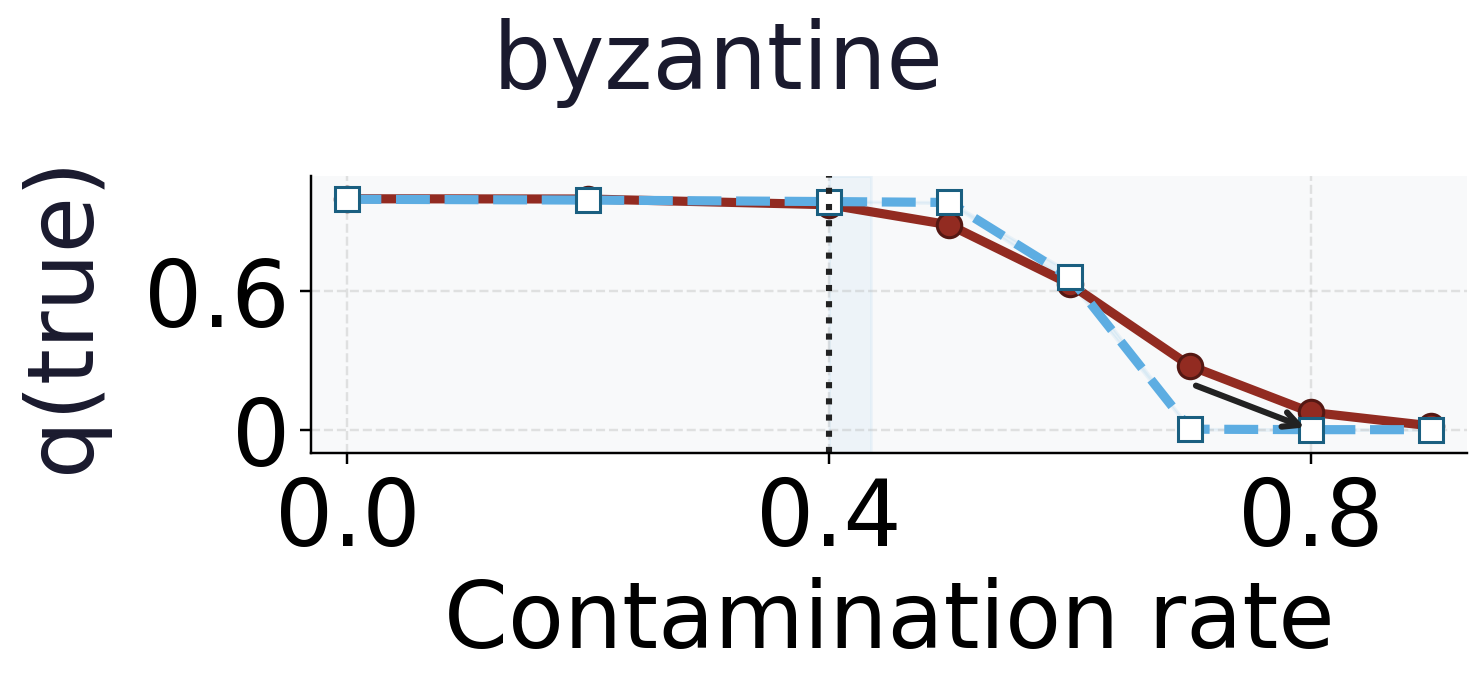
\includegraphics[keepaspectratio,width=0.98\linewidth,height=0.8\textheight,alt={byzantine: complete reference and pooled display-preset curves with their source-supplied seed bands and onset marker.}]{../figures/robustness_onset.slide-mechanism-1.png}
\refstepcounter{figure}\label{fig:robustness-onset-slide-panel-1}
\end{figure}
\end{frame}

\begin{frame}{Robustness onset by\ldots{} (part 10)}
\begin{figure}
\centering
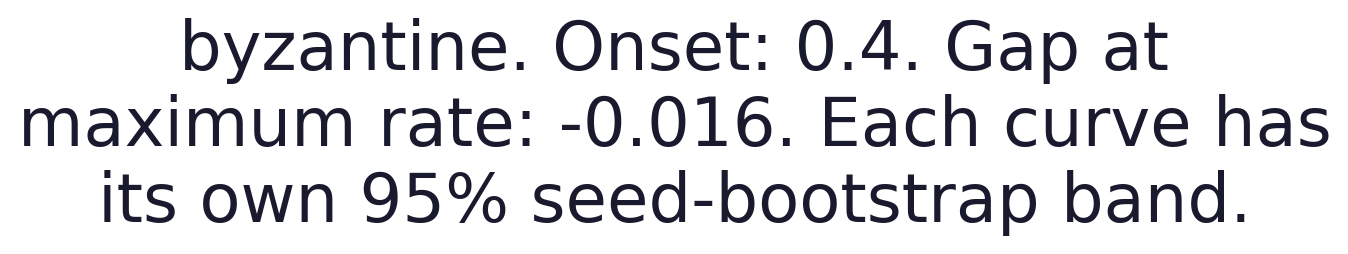
\includegraphics[keepaspectratio,width=0.98\linewidth,height=0.8\textheight,alt={byzantine. Onset: 0.4. Gap at maximum rate: -0.016. Each curve has its own 95\% seed-bootstrap band.}]{../figures/robustness_onset.slide-mechanism-1-notes.png}
\refstepcounter{figure}\label{fig:robustness-onset-slide-panel-2}
\end{figure}
\end{frame}

\begin{frame}{Robustness onset by\ldots{} (part 11)}
\begin{figure}
\centering

\includegraphics[keepaspectratio,width=0.98\linewidth,height=0.8\textheight,alt={Arrow: declared byzantine veto cliff near the penultimate rate. The onset window does not establish universal robustness.}]{../figures/robustness_onset.slide-veto-cliff.png}
\refstepcounter{figure}\label{fig:robustness-onset-slide-panel-3}
\end{figure}
\end{frame}

\begin{frame}{Robustness onset by\ldots{} (part 12)}
\begin{figure}
\centering
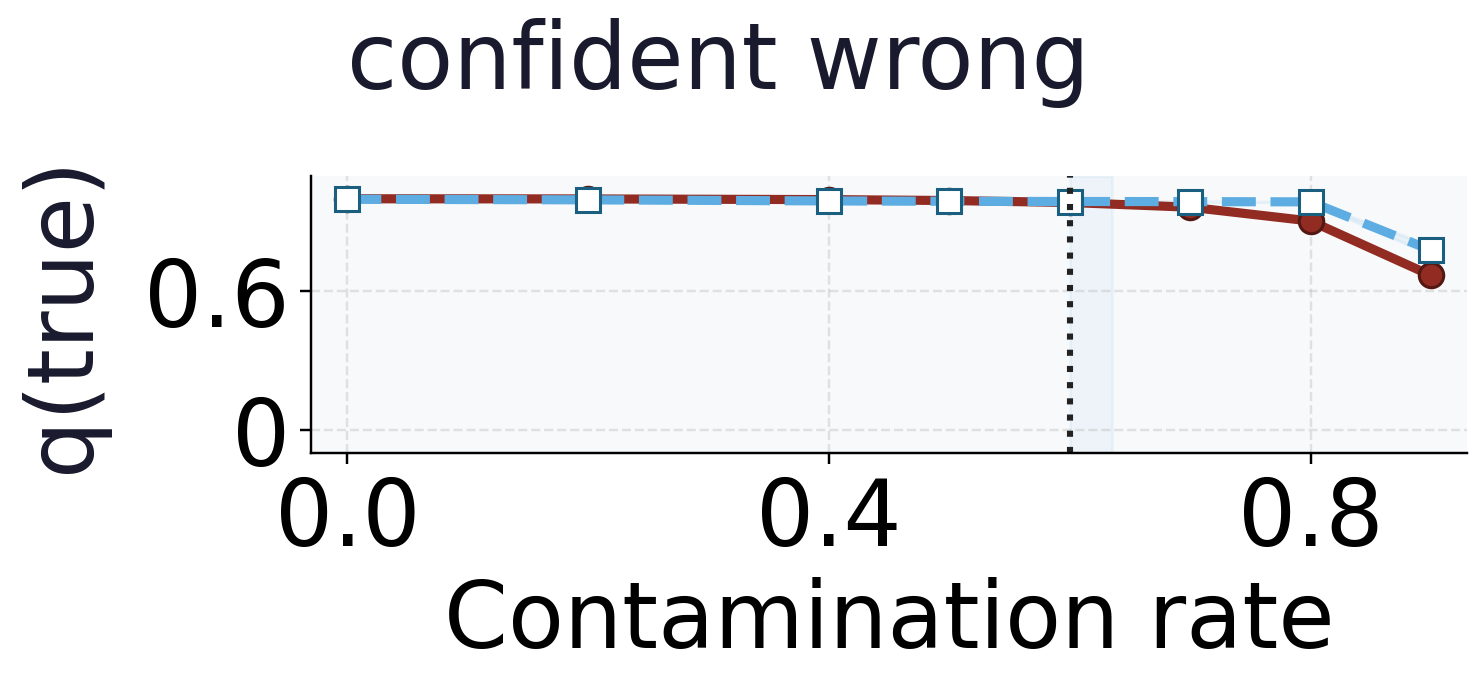
\includegraphics[keepaspectratio,width=0.98\linewidth,height=0.8\textheight,alt={confident\_wrong: complete reference and pooled display-preset curves with their source-supplied seed bands and onset marker.}]{../figures/robustness_onset.slide-mechanism-2.png}
\refstepcounter{figure}\label{fig:robustness-onset-slide-panel-4}
\end{figure}
\end{frame}

\begin{frame}{Robustness onset by\ldots{} (part 13)}
\begin{figure}
\centering
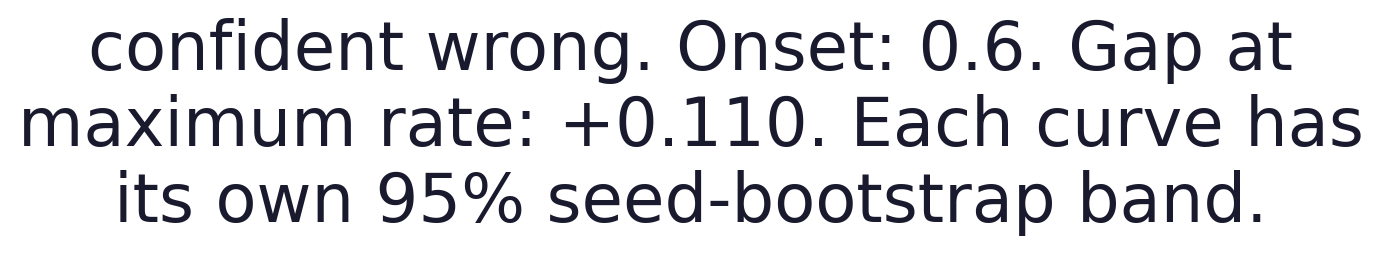
\includegraphics[keepaspectratio,width=0.98\linewidth,height=0.8\textheight,alt={confident wrong. Onset: 0.6. Gap at maximum rate: +0.110. Each curve has its own 95\% seed-bootstrap band.}]{../figures/robustness_onset.slide-mechanism-2-notes.png}
\refstepcounter{figure}\label{fig:robustness-onset-slide-panel-5}
\end{figure}
\end{frame}

\begin{frame}{Robustness onset by\ldots{} (part 14)}
\begin{figure}
\centering
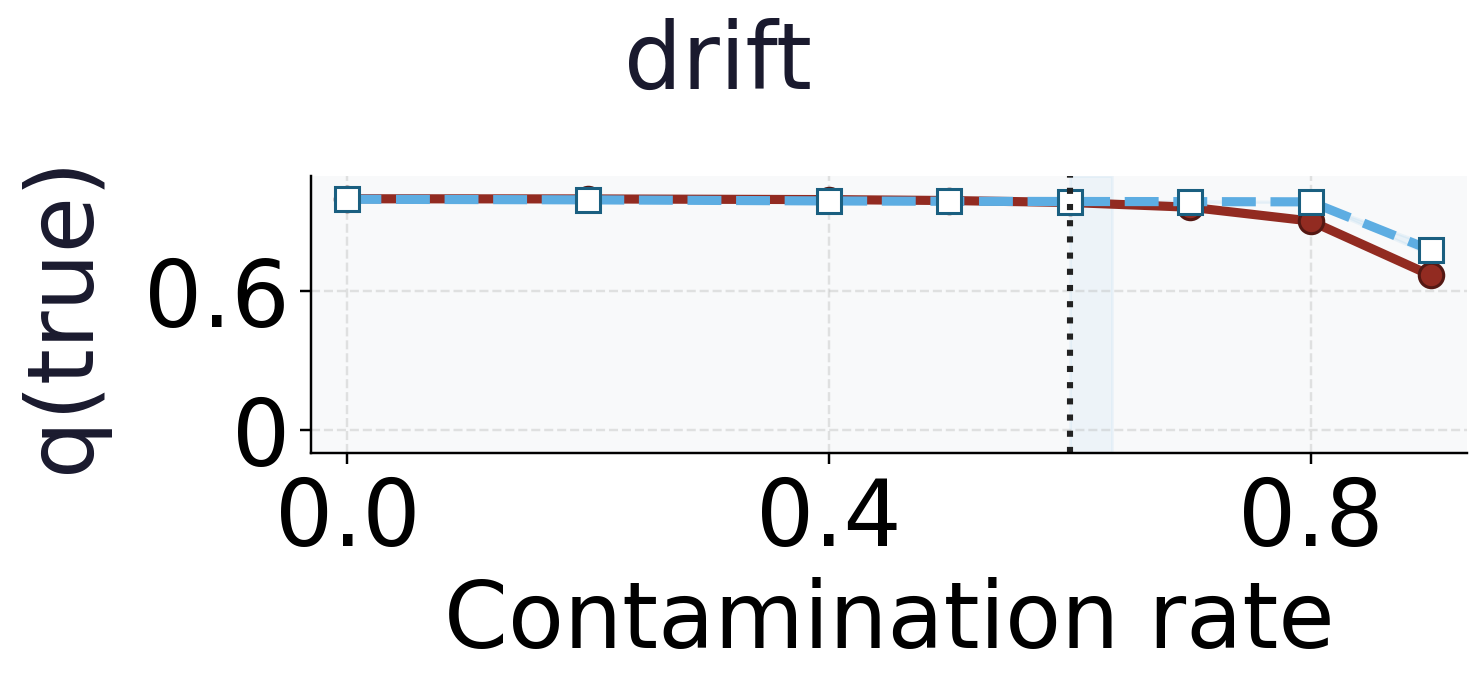
\includegraphics[keepaspectratio,width=0.98\linewidth,height=0.8\textheight,alt={drift: complete reference and pooled display-preset curves with their source-supplied seed bands and onset marker.}]{../figures/robustness_onset.slide-mechanism-3.png}
\refstepcounter{figure}\label{fig:robustness-onset-slide-panel-6}
\end{figure}
\end{frame}

\begin{frame}{Robustness onset by\ldots{} (part 15)}
\begin{figure}
\centering
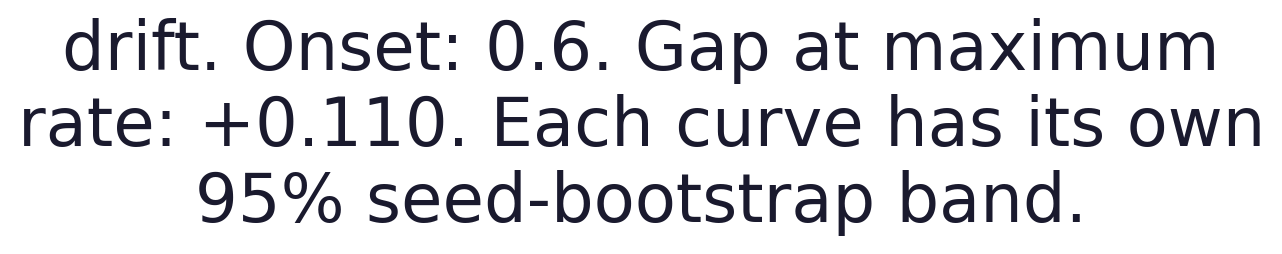
\includegraphics[keepaspectratio,width=0.98\linewidth,height=0.8\textheight,alt={drift. Onset: 0.6. Gap at maximum rate: +0.110. Each curve has its own 95\% seed-bootstrap band.}]{../figures/robustness_onset.slide-mechanism-3-notes.png}
\refstepcounter{figure}\label{fig:robustness-onset-slide-panel-7}
\end{figure}
\end{frame}

\begin{frame}{Robustness onset by\ldots{} (part 16)}
\begin{figure}
\centering
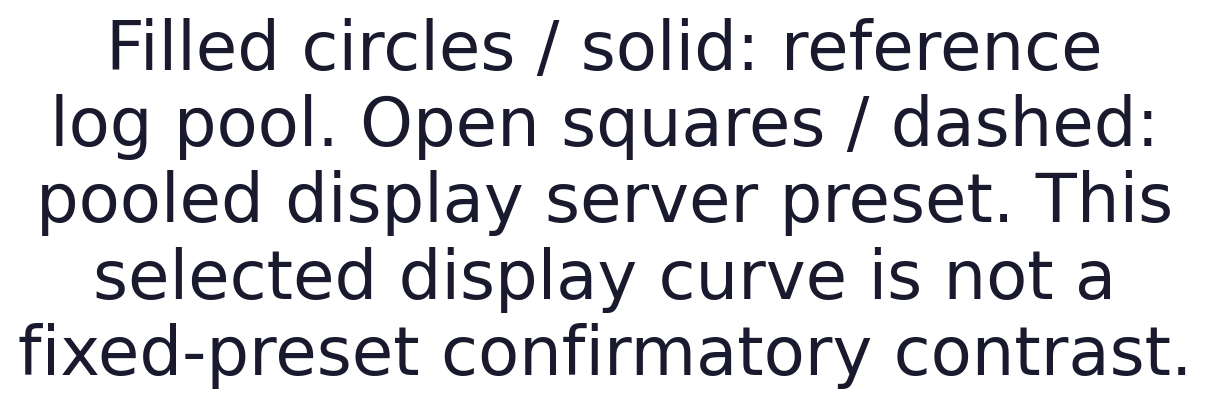
\includegraphics[keepaspectratio,width=0.98\linewidth,height=0.8\textheight,alt={Filled circles / solid: reference log pool. Open squares / dashed: pooled display server preset. This selected display curve is not a fixed-preset confirmatory contrast.}]{../figures/robustness_onset.slide-key.png}
\refstepcounter{figure}\label{fig:robustness-onset-slide-panel-8}
\end{figure}
\end{frame}

\begin{frame}{Conditional world and attack-geometry grid}
\protect\phantomsection\label{sec:supp-conditional-world}
The finite MAJ-1 characterization is now extended across 40
preregistered world/scenario cells: two hidden-state locations, two
observability levels, five attack mechanisms,
\end{frame}

\begin{frame}{Conditional world and\ldots{} (part 2)}
and two adversarial weight settings.
\end{frame}

\begin{frame}{Conditional world and\ldots{} (part 3)}
The independent unit is the seeded world/scenario row; each cell
averages 24 nested trials over 64 seeds before the matched contrast is
formed. The primary estimand is naive true-state error minus robust
true-state error,
\end{frame}

\begin{frame}{Conditional world and\ldots{} (part 4)}
so a positive value means the robust heuristic assigns more true-state
mass in that finite cell.
\end{frame}

\begin{frame}[fragile]{Conditional world and\ldots{} (part 5)}
The robustness-zero control is pass, and the report remains explicitly
labelled \texttt{conditional\_finite\_grid}. The resulting conditional
surface is shown in fig.~24.
\end{frame}

\begin{frame}{Conditional world and\ldots{} (part 6)}
\begin{figure}
\centering
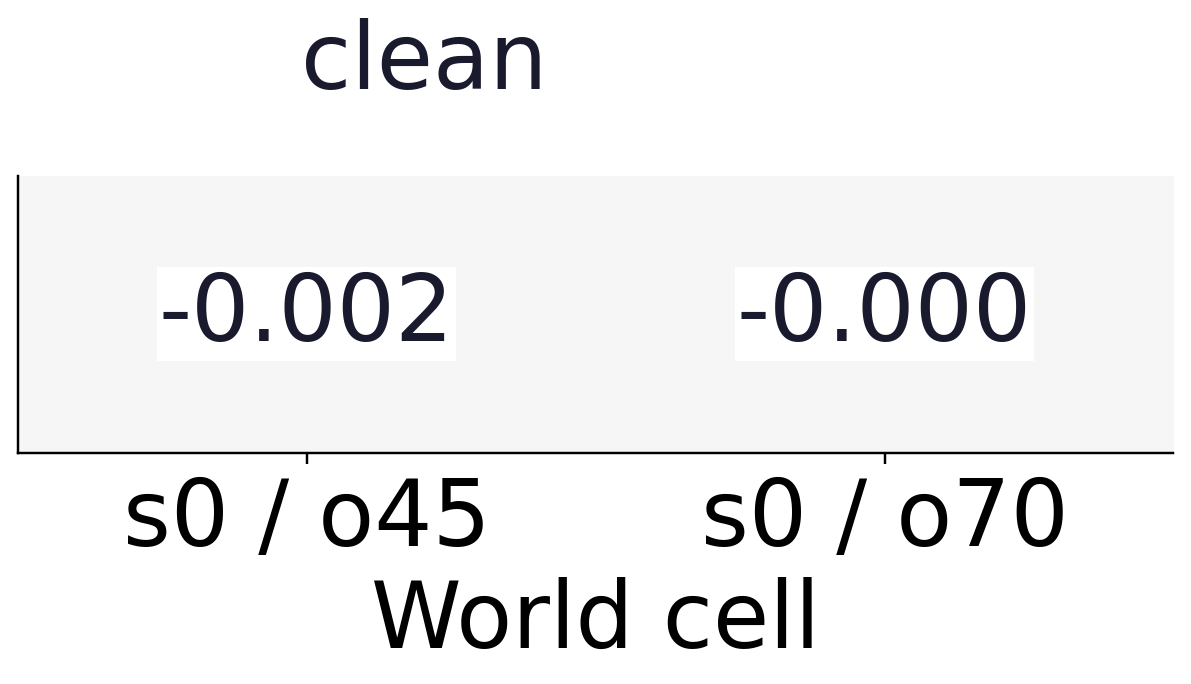
\includegraphics[keepaspectratio,width=0.98\linewidth,height=0.8\textheight,alt={clean: signed seed-level contrasts for the two displayed world cells; fixed symmetric color scale.}]{../figures/conditional_world.slide-attack-1-cells-1-2.png}
\refstepcounter{figure}\label{fig:conditional-world-slide-panel-1}
\end{figure}
\end{frame}

\begin{frame}{Conditional world and\ldots{} (part 7)}
\begin{figure}
\centering
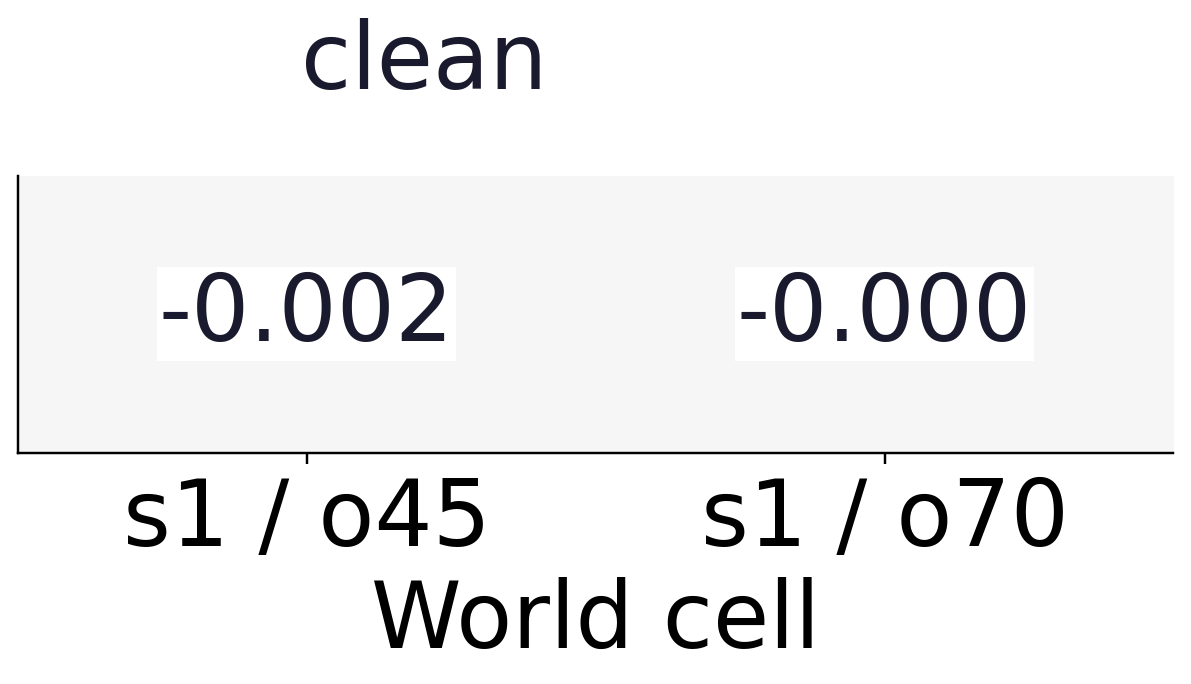
\includegraphics[keepaspectratio,width=0.98\linewidth,height=0.8\textheight,alt={clean: signed seed-level contrasts for the two displayed world cells; fixed symmetric color scale.}]{../figures/conditional_world.slide-attack-1-cells-3-4.png}
\refstepcounter{figure}\label{fig:conditional-world-slide-panel-2}
\end{figure}
\end{frame}

\begin{frame}{Conditional world and\ldots{} (part 8)}
\begin{figure}
\centering
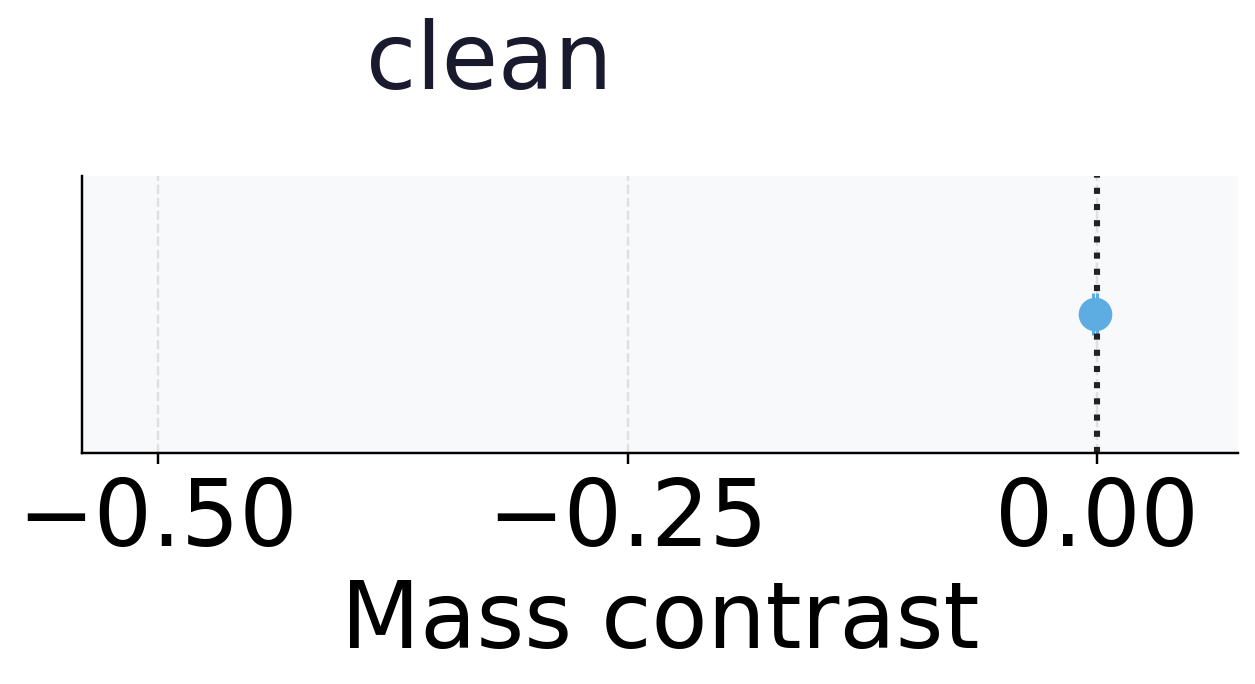
\includegraphics[keepaspectratio,width=0.98\linewidth,height=0.8\textheight,alt={clean: finite-grid mean with asymmetric capped minimum-to-maximum range on the common contrast scale.}]{../figures/conditional_world.slide-attack-1-range.png}
\refstepcounter{figure}\label{fig:conditional-world-slide-panel-3}
\end{figure}
\end{frame}

\begin{frame}{Conditional world and\ldots{} (part 9)}
\begin{figure}
\centering
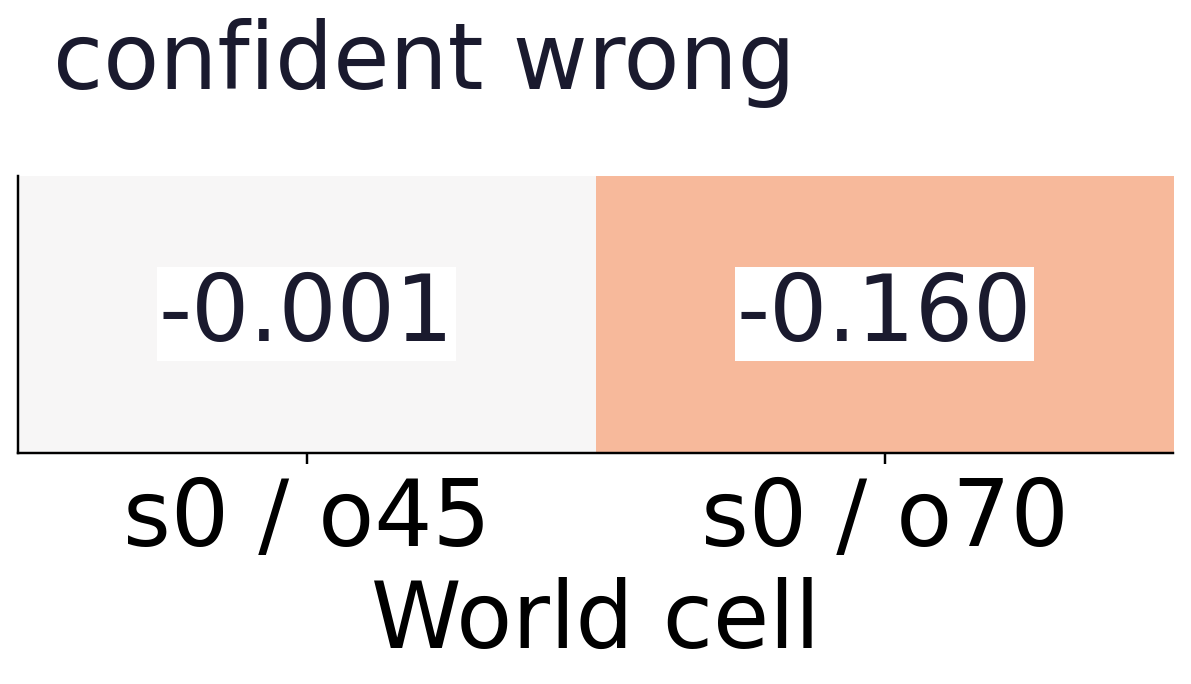
\includegraphics[keepaspectratio,width=0.98\linewidth,height=0.8\textheight,alt={confident\_wrong: signed seed-level contrasts for the two displayed world cells; fixed symmetric color scale.}]{../figures/conditional_world.slide-attack-2-cells-1-2.png}
\refstepcounter{figure}\label{fig:conditional-world-slide-panel-4}
\end{figure}
\end{frame}

\begin{frame}{Conditional world and\ldots{} (part 10)}
\begin{figure}
\centering
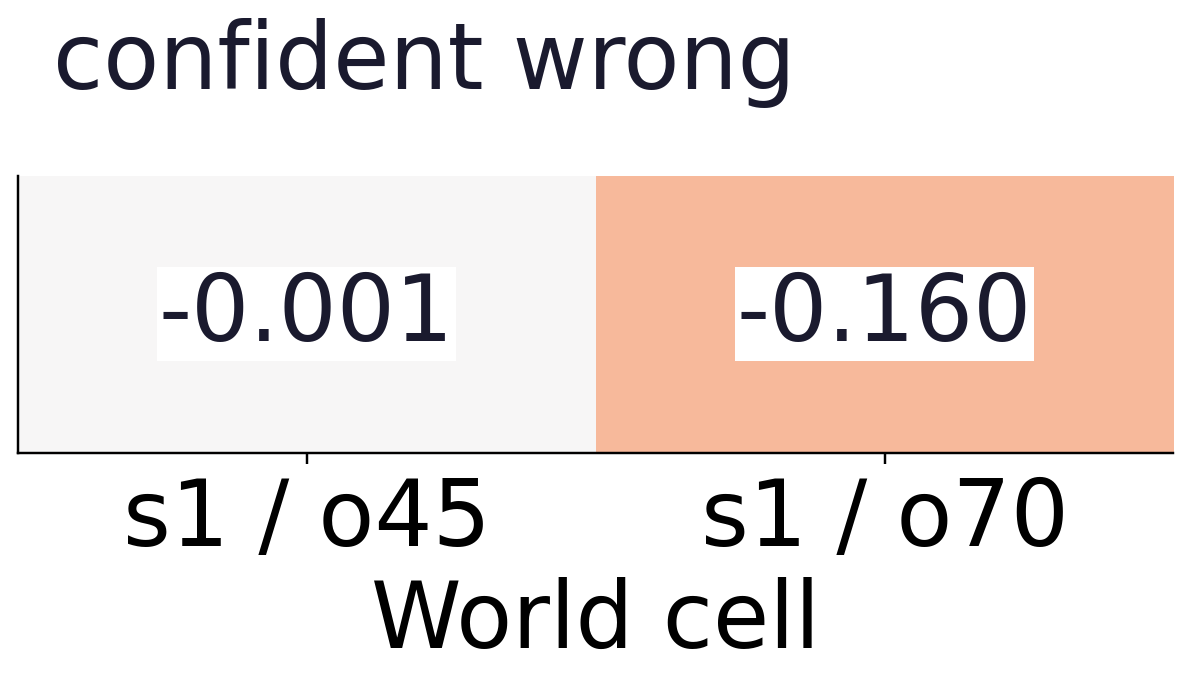
\includegraphics[keepaspectratio,width=0.98\linewidth,height=0.8\textheight,alt={confident\_wrong: signed seed-level contrasts for the two displayed world cells; fixed symmetric color scale.}]{../figures/conditional_world.slide-attack-2-cells-3-4.png}
\refstepcounter{figure}\label{fig:conditional-world-slide-panel-5}
\end{figure}
\end{frame}

\begin{frame}{Conditional world and\ldots{} (part 11)}
\begin{figure}
\centering
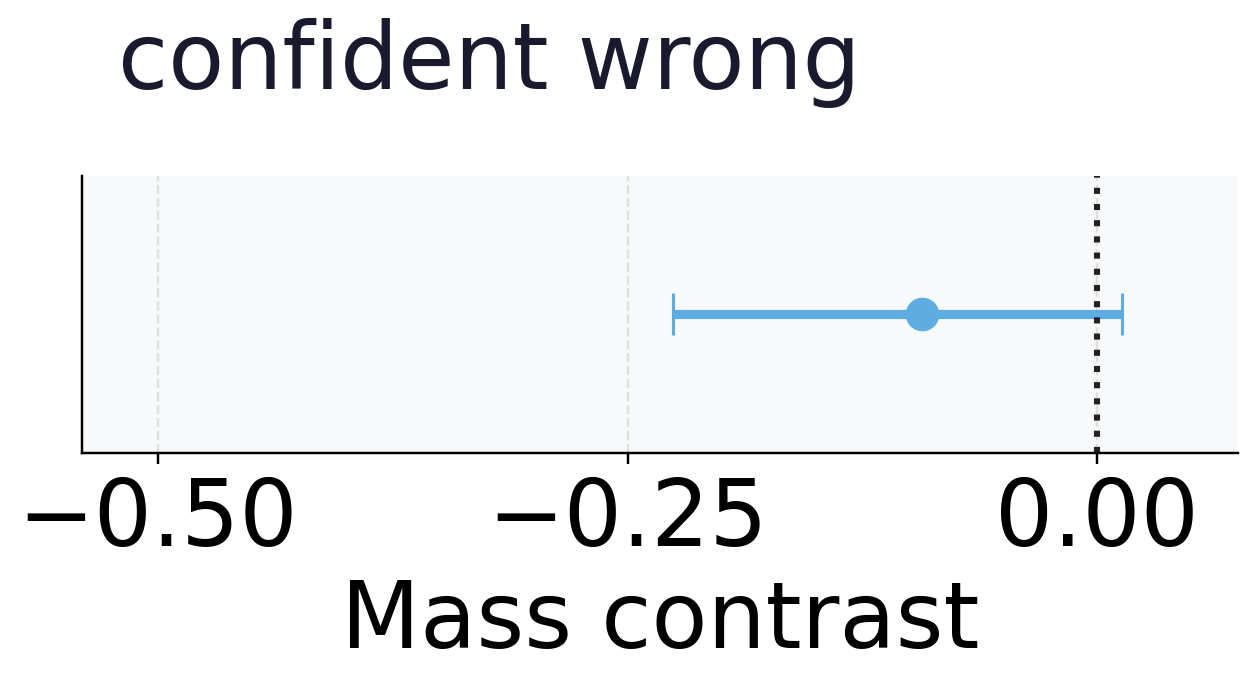
\includegraphics[keepaspectratio,width=0.98\linewidth,height=0.8\textheight,alt={confident\_wrong: finite-grid mean with asymmetric capped minimum-to-maximum range on the common contrast scale.}]{../figures/conditional_world.slide-attack-2-range.png}
\refstepcounter{figure}\label{fig:conditional-world-slide-panel-6}
\end{figure}
\end{frame}

\begin{frame}{Conditional world and\ldots{} (part 12)}
\begin{figure}
\centering
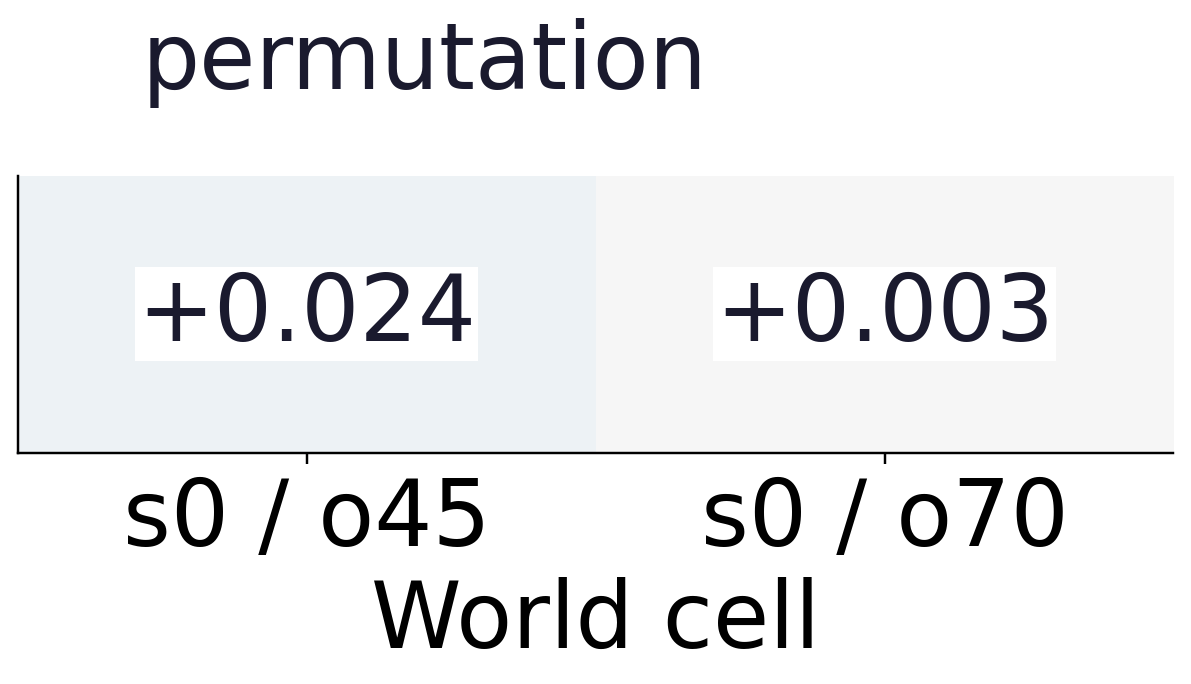
\includegraphics[keepaspectratio,width=0.98\linewidth,height=0.8\textheight,alt={permutation: signed seed-level contrasts for the two displayed world cells; fixed symmetric color scale.}]{../figures/conditional_world.slide-attack-3-cells-1-2.png}
\refstepcounter{figure}\label{fig:conditional-world-slide-panel-7}
\end{figure}
\end{frame}

\begin{frame}{Conditional world and\ldots{} (part 13)}
\begin{figure}
\centering
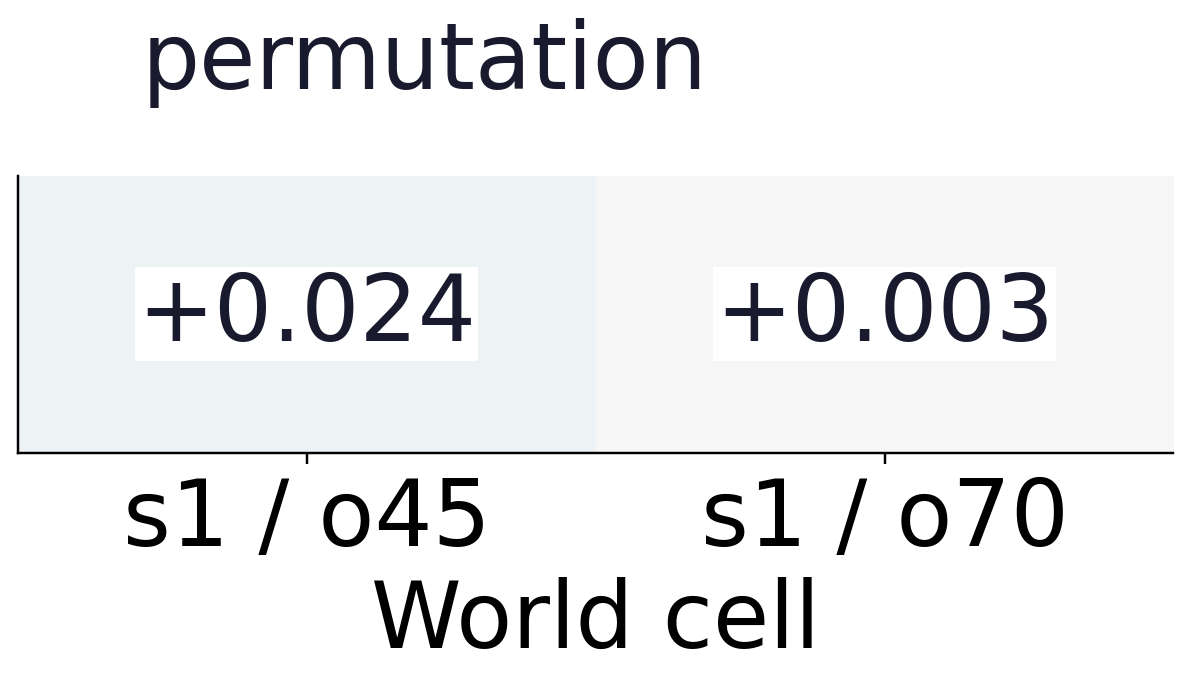
\includegraphics[keepaspectratio,width=0.98\linewidth,height=0.8\textheight,alt={permutation: signed seed-level contrasts for the two displayed world cells; fixed symmetric color scale.}]{../figures/conditional_world.slide-attack-3-cells-3-4.png}
\refstepcounter{figure}\label{fig:conditional-world-slide-panel-8}
\end{figure}
\end{frame}

\begin{frame}{Conditional world and\ldots{} (part 14)}
\begin{figure}
\centering
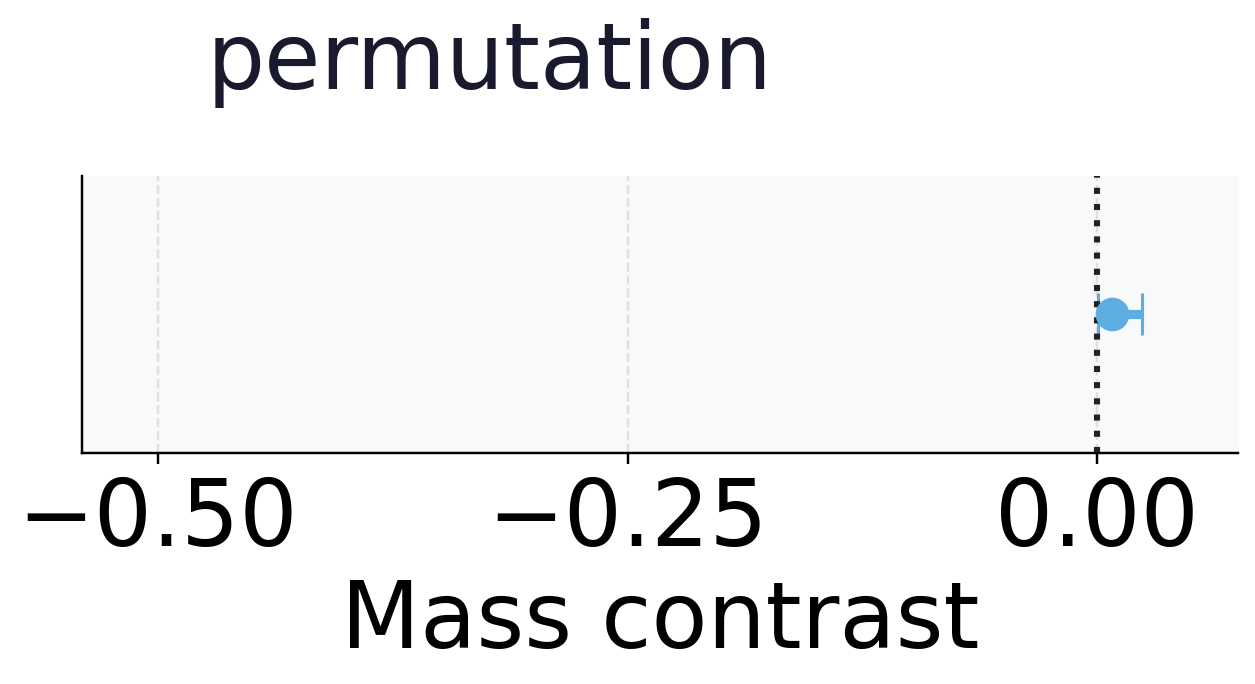
\includegraphics[keepaspectratio,width=0.98\linewidth,height=0.8\textheight,alt={permutation: finite-grid mean with asymmetric capped minimum-to-maximum range on the common contrast scale.}]{../figures/conditional_world.slide-attack-3-range.png}
\refstepcounter{figure}\label{fig:conditional-world-slide-panel-9}
\end{figure}
\end{frame}

\begin{frame}{Conditional world and\ldots{} (part 15)}
\begin{figure}
\centering
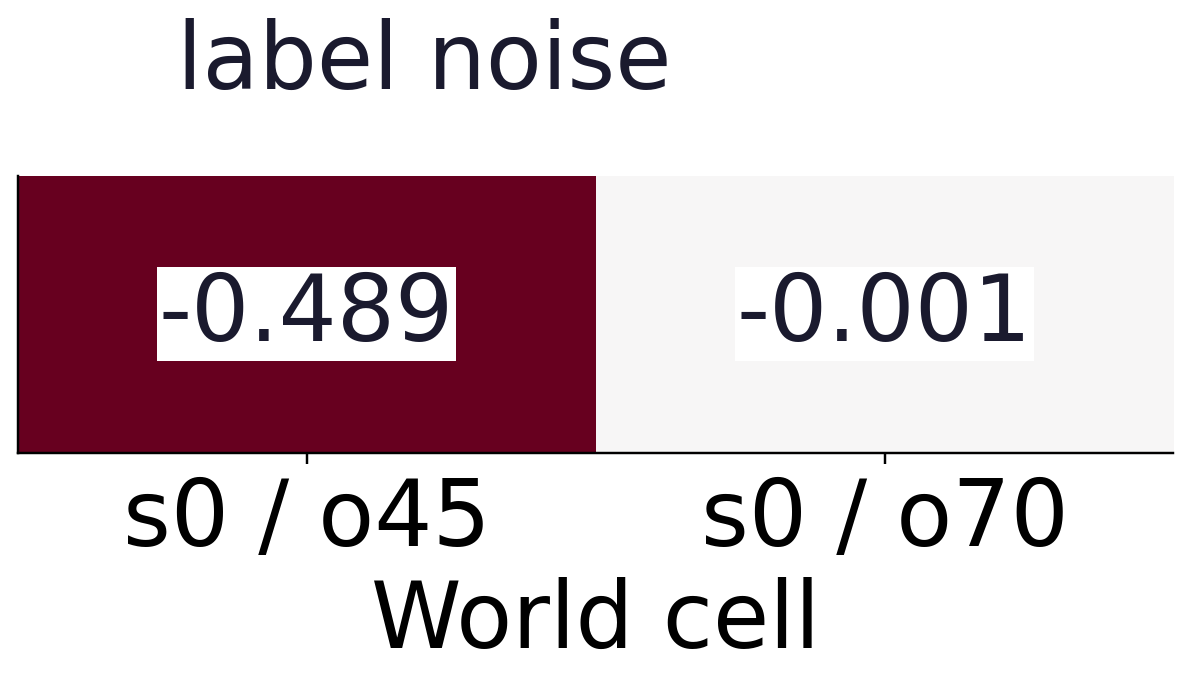
\includegraphics[keepaspectratio,width=0.98\linewidth,height=0.8\textheight,alt={label\_noise: signed seed-level contrasts for the two displayed world cells; fixed symmetric color scale.}]{../figures/conditional_world.slide-attack-4-cells-1-2.png}
\refstepcounter{figure}\label{fig:conditional-world-slide-panel-10}
\end{figure}
\end{frame}

\begin{frame}{Conditional world and\ldots{} (part 16)}
\begin{figure}
\centering
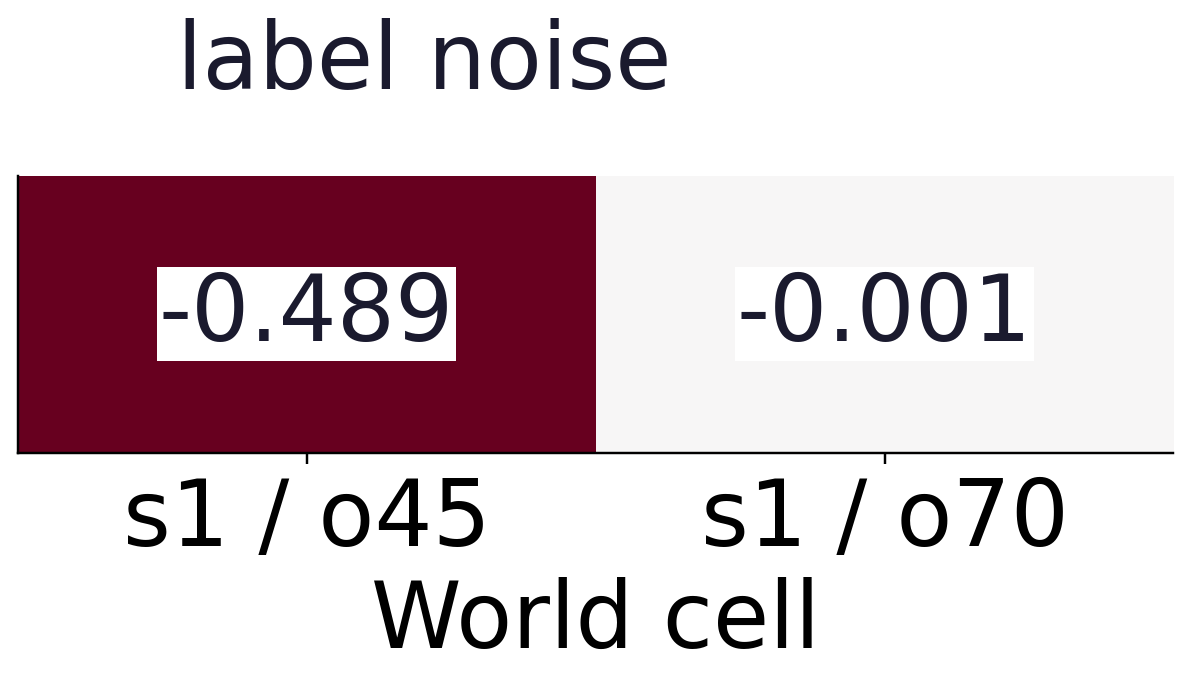
\includegraphics[keepaspectratio,width=0.98\linewidth,height=0.8\textheight,alt={label\_noise: signed seed-level contrasts for the two displayed world cells; fixed symmetric color scale.}]{../figures/conditional_world.slide-attack-4-cells-3-4.png}
\refstepcounter{figure}\label{fig:conditional-world-slide-panel-11}
\end{figure}
\end{frame}

\begin{frame}{Conditional world and\ldots{} (part 17)}
\begin{figure}
\centering
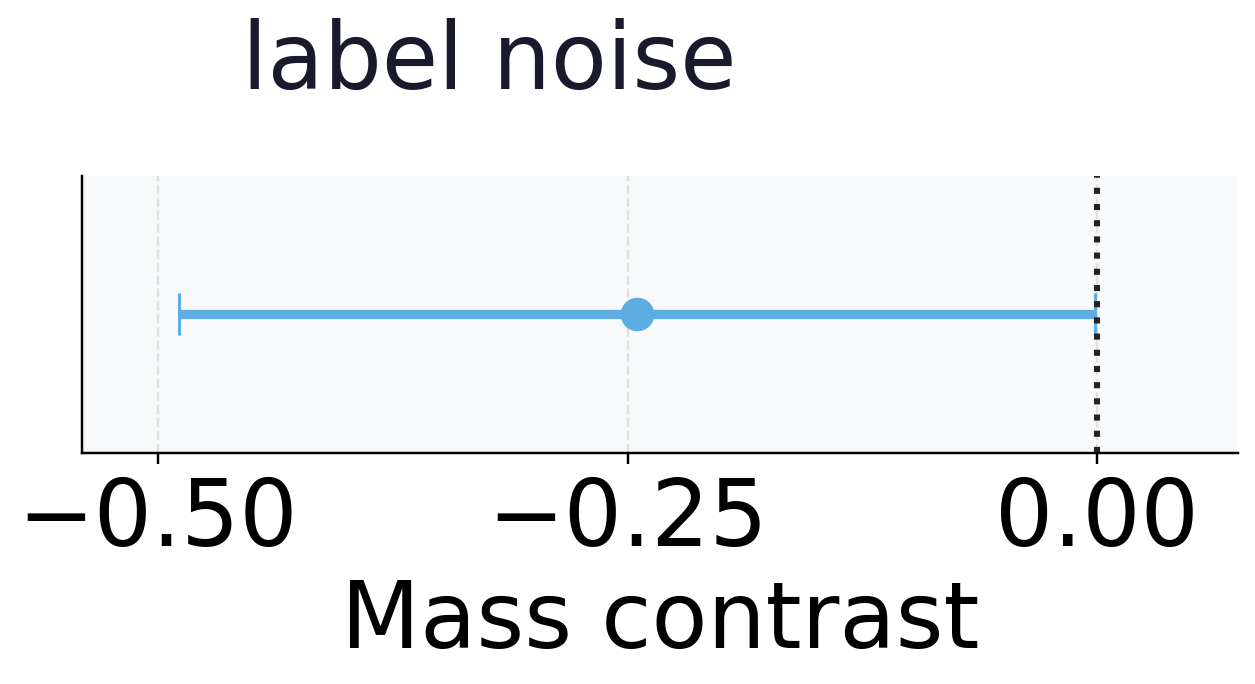
\includegraphics[keepaspectratio,width=0.98\linewidth,height=0.8\textheight,alt={label\_noise: finite-grid mean with asymmetric capped minimum-to-maximum range on the common contrast scale.}]{../figures/conditional_world.slide-attack-4-range.png}
\refstepcounter{figure}\label{fig:conditional-world-slide-panel-12}
\end{figure}
\end{frame}

\begin{frame}{Conditional world and\ldots{} (part 18)}
\begin{figure}
\centering
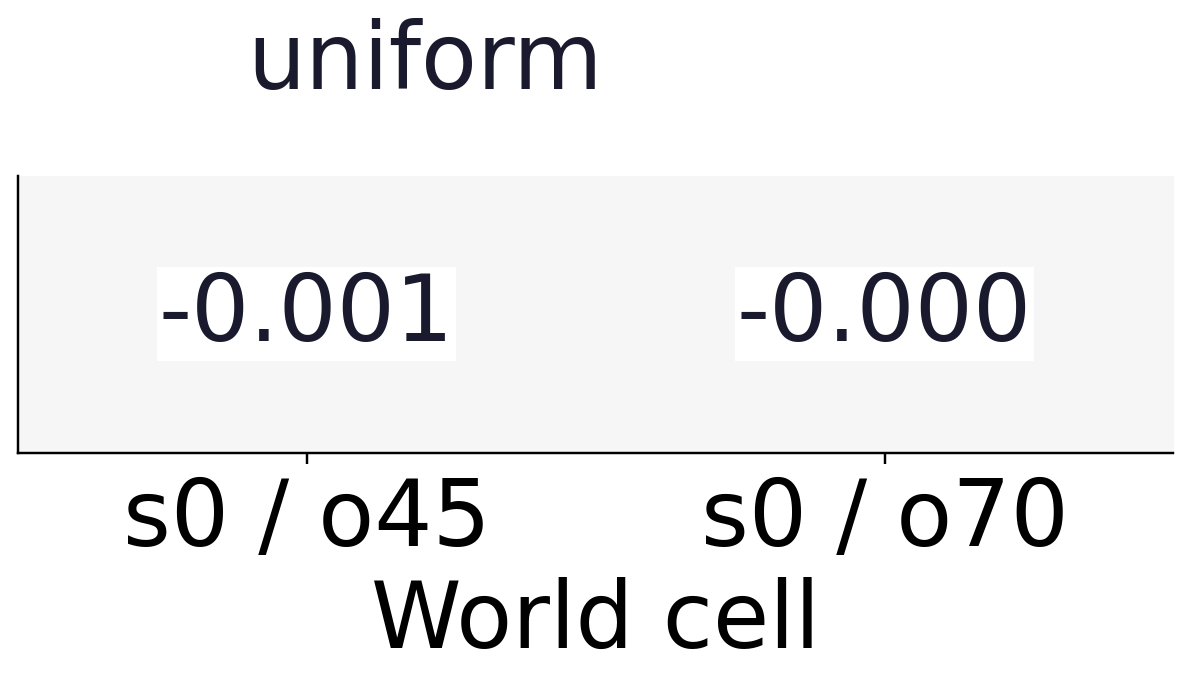
\includegraphics[keepaspectratio,width=0.98\linewidth,height=0.8\textheight,alt={uniform: signed seed-level contrasts for the two displayed world cells; fixed symmetric color scale.}]{../figures/conditional_world.slide-attack-5-cells-1-2.png}
\refstepcounter{figure}\label{fig:conditional-world-slide-panel-13}
\end{figure}
\end{frame}

\begin{frame}{Conditional world and\ldots{} (part 19)}
\begin{figure}
\centering
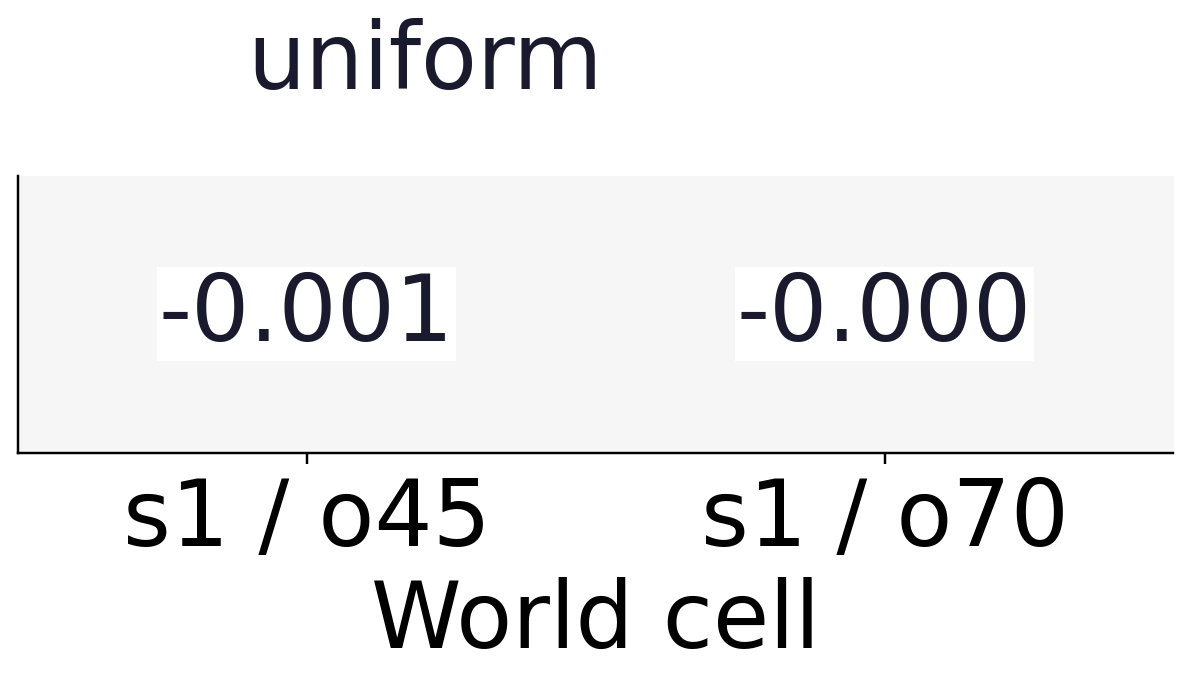
\includegraphics[keepaspectratio,width=0.98\linewidth,height=0.8\textheight,alt={uniform: signed seed-level contrasts for the two displayed world cells; fixed symmetric color scale.}]{../figures/conditional_world.slide-attack-5-cells-3-4.png}
\refstepcounter{figure}\label{fig:conditional-world-slide-panel-14}
\end{figure}
\end{frame}

\begin{frame}{Conditional world and\ldots{} (part 20)}
\begin{figure}
\centering
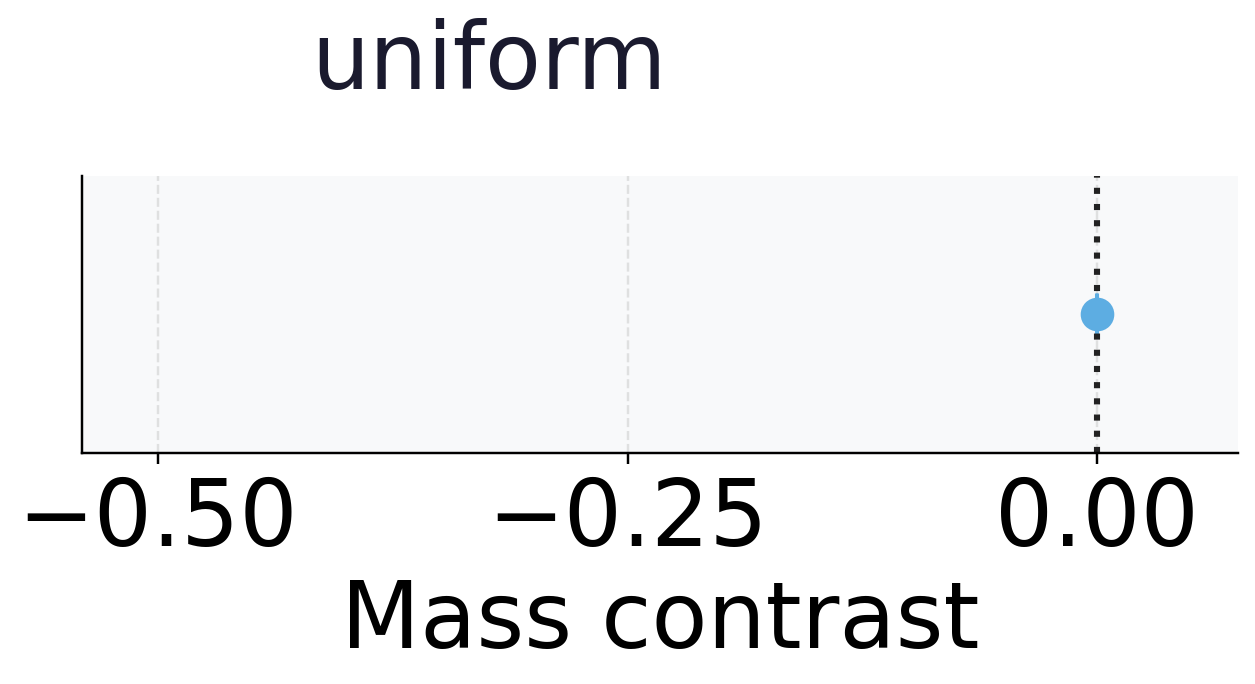
\includegraphics[keepaspectratio,width=0.98\linewidth,height=0.8\textheight,alt={uniform: finite-grid mean with asymmetric capped minimum-to-maximum range on the common contrast scale.}]{../figures/conditional_world.slide-attack-5-range.png}
\refstepcounter{figure}\label{fig:conditional-world-slide-panel-15}
\end{figure}
\end{frame}

\begin{frame}{Conditional world and\ldots{} (part 21)}
\begin{figure}
\centering

\includegraphics[keepaspectratio,width=0.98\linewidth,height=0.8\textheight,alt={Seed-level true-state-mass contrast: naive error minus robust error. Positive values favor the heuristic on the declared finite grid.}]{../figures/conditional_world.slide-key.png}
\refstepcounter{figure}\label{fig:conditional-world-slide-panel-16}
\end{figure}
\end{frame}

\begin{frame}{Conditional world and\ldots{} (part 22)}
\begin{figure}
\centering
\includegraphics[keepaspectratio,width=0.98\linewidth,height=0.8\textheight,alt={Heatmap: adversary weight 1. State s0/s1; observability o45/o70. Common color scale: {[}-0.4889, 0.4889{]}. Every cell prints its signed mean.}]{../figures/conditional_world.slide-grid.png}
\refstepcounter{figure}\label{fig:conditional-world-slide-panel-17}
\end{figure}
\end{frame}

\begin{frame}{Conditional world and\ldots{} (part 23)}
\begin{figure}
\centering
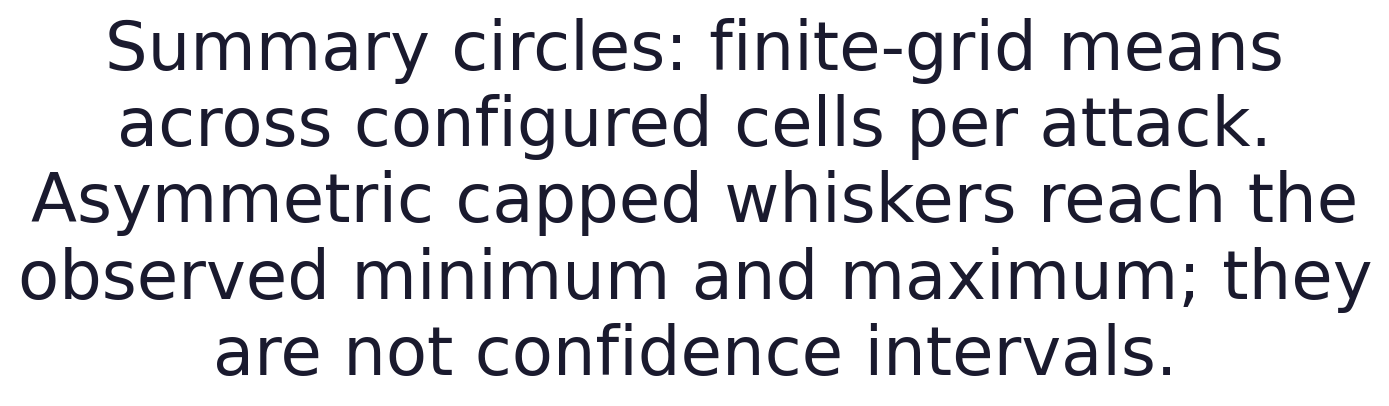
\includegraphics[keepaspectratio,width=0.98\linewidth,height=0.8\textheight,alt={Summary circles: finite-grid means across configured cells per attack. Asymmetric capped whiskers reach the observed minimum and maximum; they are not confidence intervals.}]{../figures/conditional_world.slide-ranges.png}
\refstepcounter{figure}\label{fig:conditional-world-slide-panel-18}
\end{figure}
\end{frame}

\begin{frame}{Conditional world and\ldots{} (part 24)}
\begin{figure}
\centering
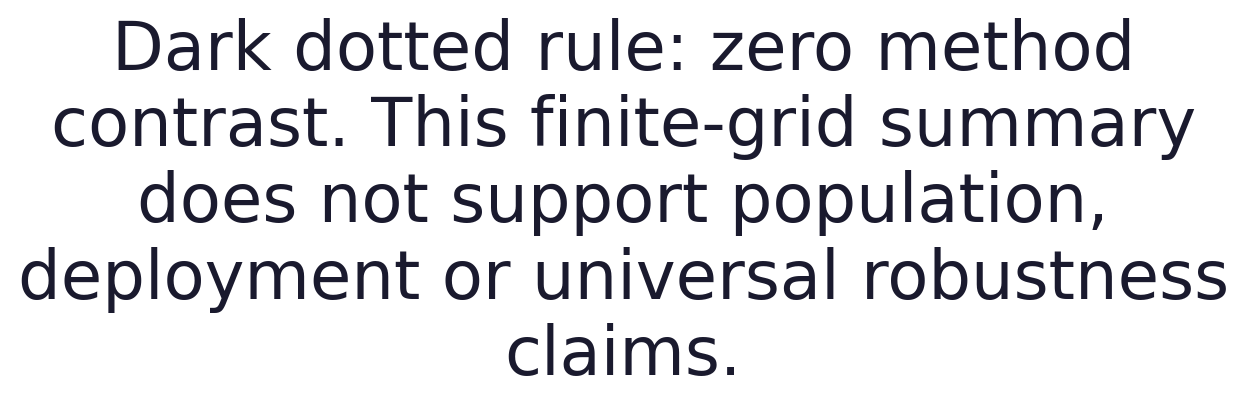
\includegraphics[keepaspectratio,width=0.98\linewidth,height=0.8\textheight,alt={Dark dotted rule: zero method contrast. This finite-grid summary does not support population, deployment or universal robustness claims.}]{../figures/conditional_world.slide-scope.png}
\refstepcounter{figure}\label{fig:conditional-world-slide-panel-19}
\end{figure}
\end{frame}

\begin{frame}{Proper scores and calibration controls}
\protect\phantomsection\label{sec:supp-belief-quality}
Argmax accuracy does not distinguish a cautious posterior from an
overconfident one. The scoring extension therefore pre-registers the
paired seed-level categorical log-score difference between naive and
robust consensus beliefs as its primary belief-quality estimand.
\end{frame}

\begin{frame}{Proper scores and\ldots{} (part 2)}
The Brier score and equal-width expected calibration error are secondary
diagnostics; higher log score and lower Brier/ECE are better. Agents and
trials remain nested within the seed.
\end{frame}

\begin{frame}[fragile]{Proper scores and\ldots{} (part 3)}
The report also includes three negative controls: an oracle, a uniform
belief, and a confidently wrong belief. Their expected score ordering is
checked before any method contrast is interpreted: oracle \textgreater{}
uniform \textgreater{} confidently wrong under the clipped log score.
The control ordering gate is \texttt{pass},
\end{frame}

\begin{frame}[fragile]{Proper scores and\ldots{} (part 4)}
and the confidently-wrong-versus-uniform control is \texttt{pass}, using
64 independent seeds and 24 nested trials per seed. The diagnostic is
shown in fig.~25.
\end{frame}

\begin{frame}{Proper scores and\ldots{} (part 5)}
\begin{figure}
\centering
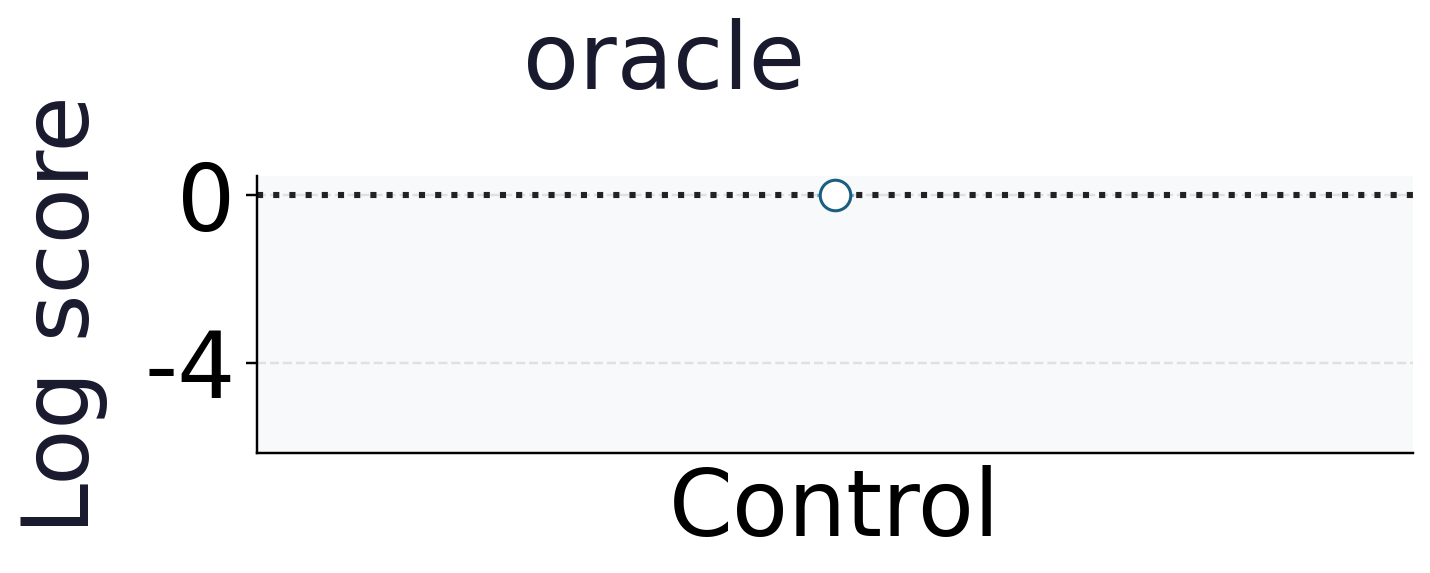
\includegraphics[keepaspectratio,width=0.98\linewidth,height=0.8\textheight,alt={oracle: mean categorical log score and its seed-bootstrap interval on the common nats scale.}]{../figures/belief_quality.slide-oracle-score.png}
\refstepcounter{figure}\label{fig:belief-quality-slide-panel-1}
\end{figure}
\end{frame}

\begin{frame}{Proper scores and\ldots{} (part 6)}
\begin{figure}
\centering
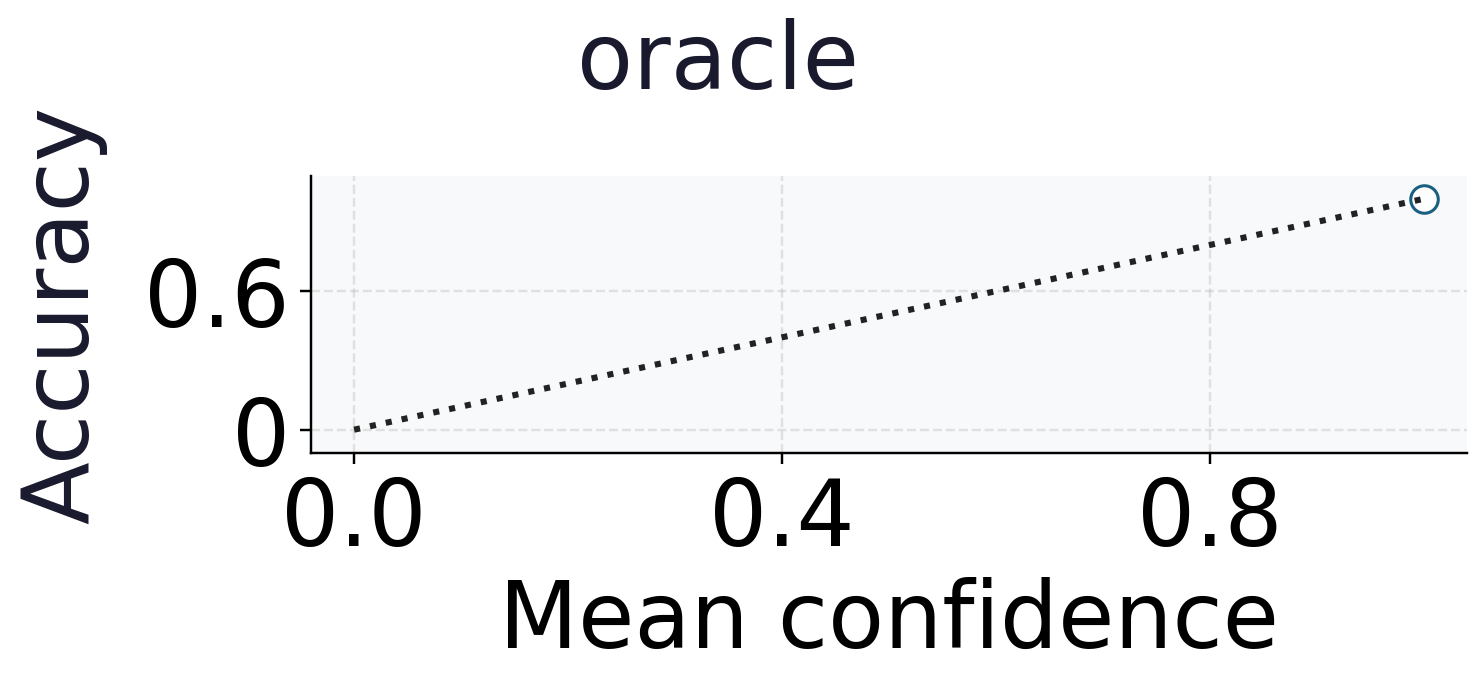
\includegraphics[keepaspectratio,width=0.98\linewidth,height=0.8\textheight,alt={oracle: every finite reliability-bin confidence and accuracy, with the perfect-calibration identity reference.}]{../figures/belief_quality.slide-oracle-reliability.png}
\refstepcounter{figure}\label{fig:belief-quality-slide-panel-2}
\end{figure}
\end{frame}

\begin{frame}{Proper scores and\ldots{} (part 7)}
\begin{figure}
\centering
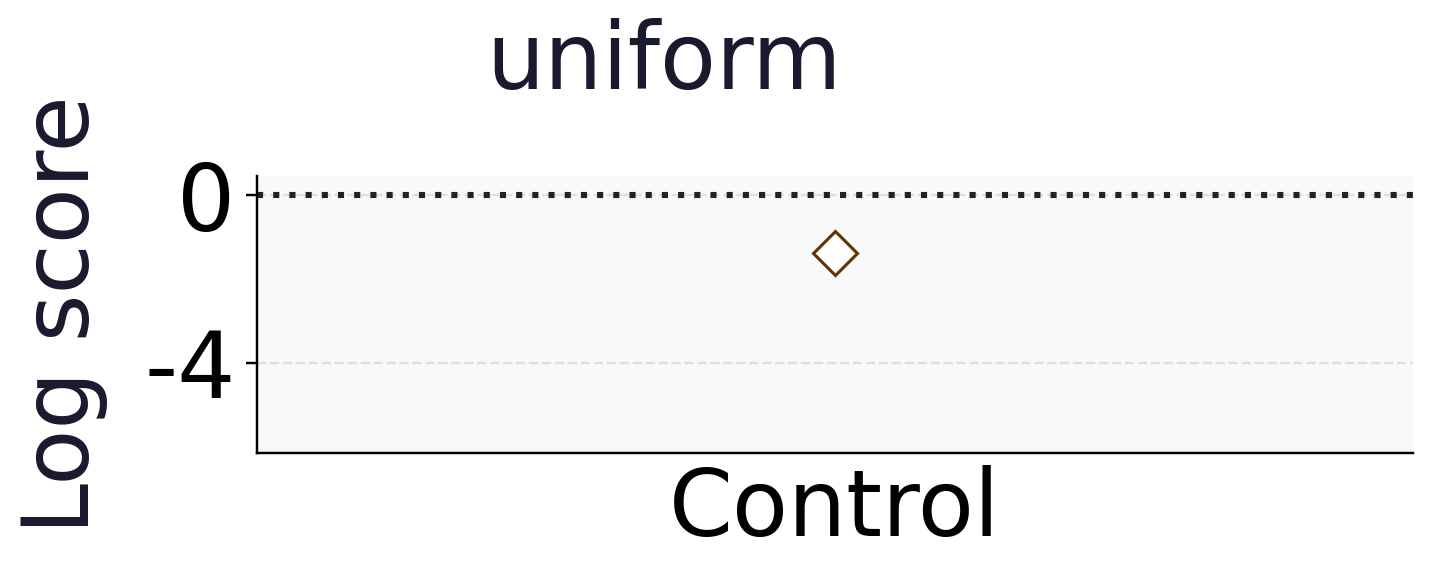
\includegraphics[keepaspectratio,width=0.98\linewidth,height=0.8\textheight,alt={uniform: mean categorical log score and its seed-bootstrap interval on the common nats scale.}]{../figures/belief_quality.slide-uniform-score.png}
\refstepcounter{figure}\label{fig:belief-quality-slide-panel-3}
\end{figure}
\end{frame}

\begin{frame}{Proper scores and\ldots{} (part 8)}
\begin{figure}
\centering
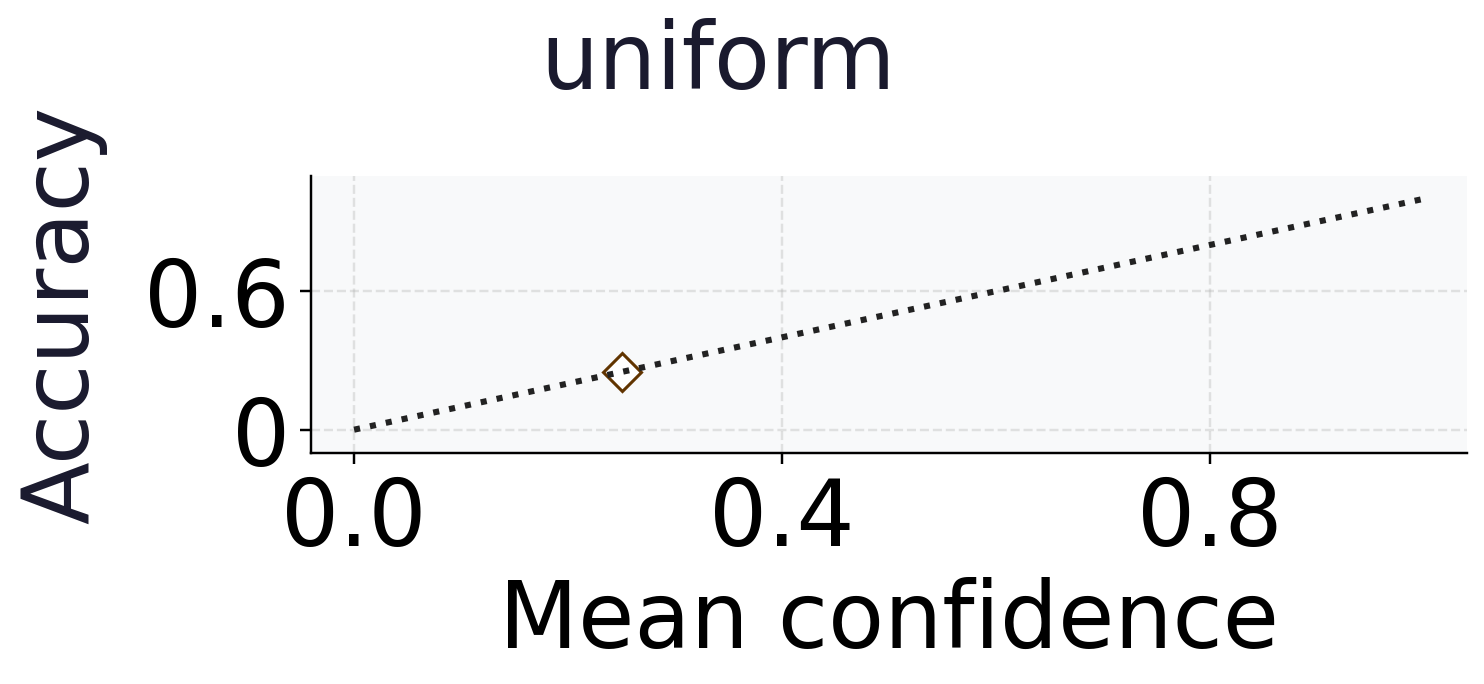
\includegraphics[keepaspectratio,width=0.98\linewidth,height=0.8\textheight,alt={uniform: every finite reliability-bin confidence and accuracy, with the perfect-calibration identity reference.}]{../figures/belief_quality.slide-uniform-reliability.png}
\refstepcounter{figure}\label{fig:belief-quality-slide-panel-4}
\end{figure}
\end{frame}

\begin{frame}{Proper scores and\ldots{} (part 9)}
\begin{figure}
\centering
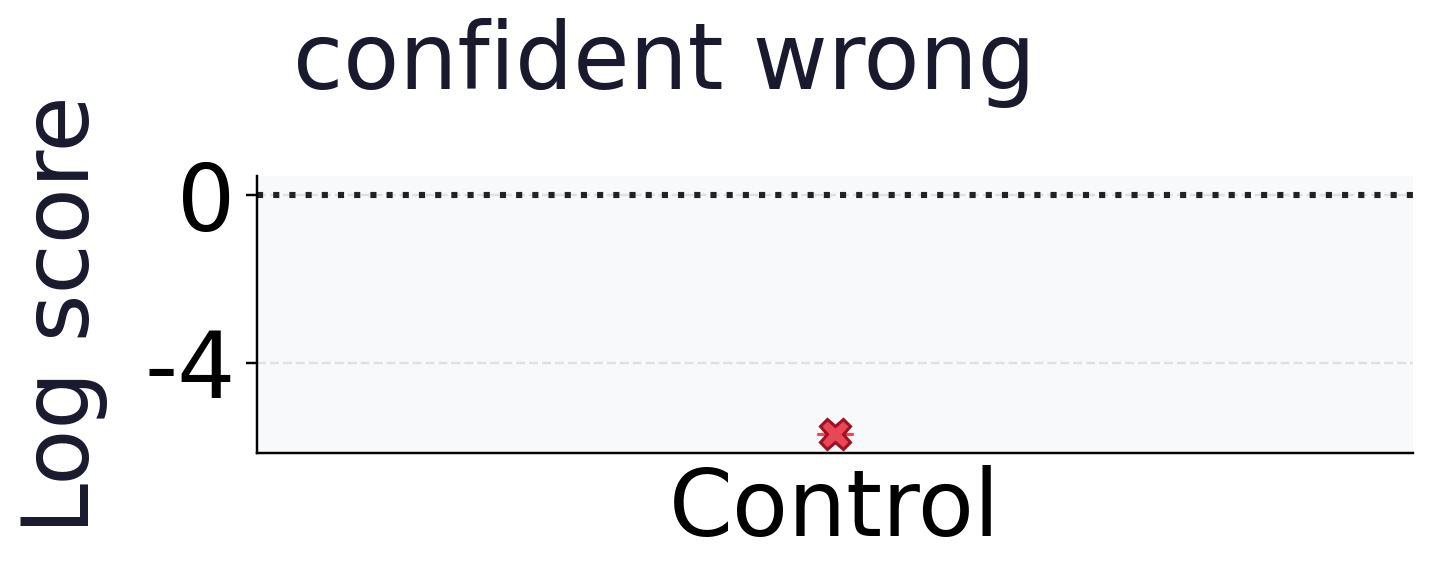
\includegraphics[keepaspectratio,width=0.98\linewidth,height=0.8\textheight,alt={confident wrong: mean categorical log score and its seed-bootstrap interval on the common nats scale.}]{../figures/belief_quality.slide-confident-wrong-score.png}
\refstepcounter{figure}\label{fig:belief-quality-slide-panel-5}
\end{figure}
\end{frame}

\begin{frame}{Proper scores and\ldots{} (part 10)}
\begin{figure}
\centering
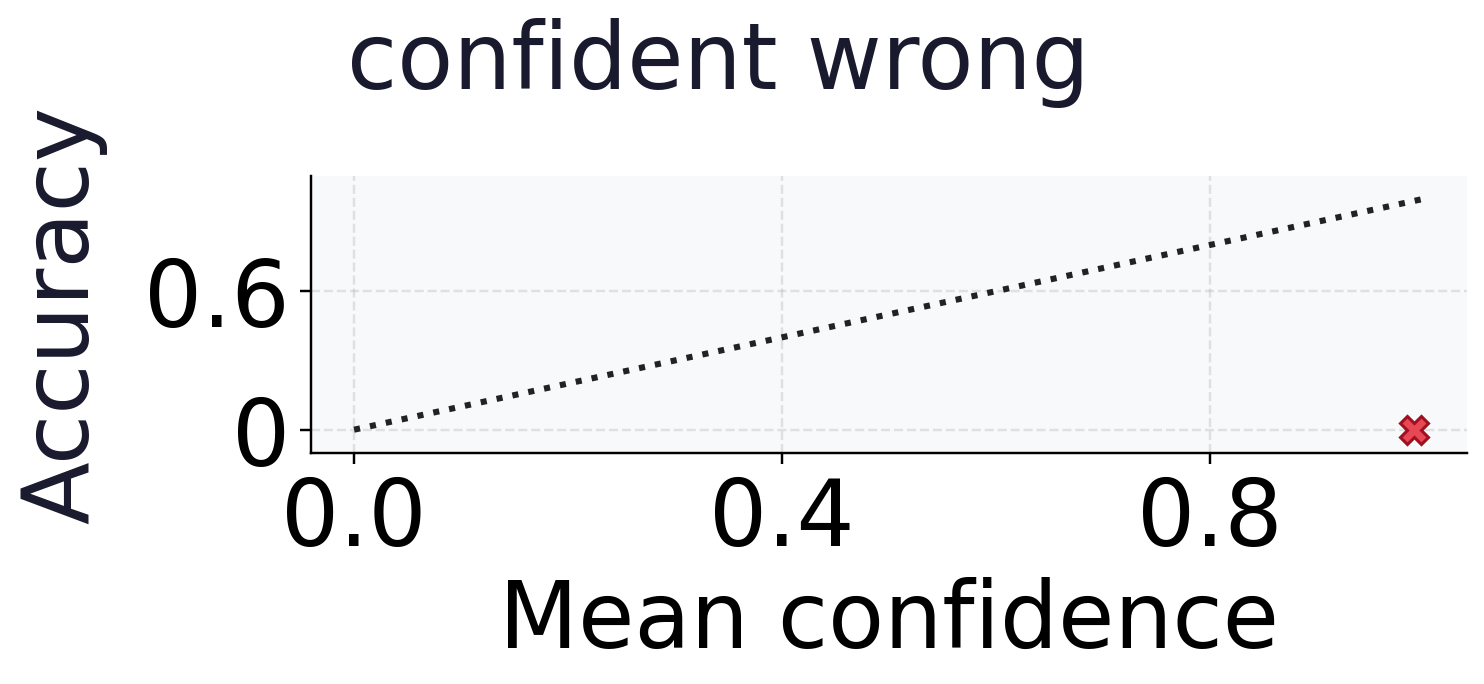
\includegraphics[keepaspectratio,width=0.98\linewidth,height=0.8\textheight,alt={confident wrong: every finite reliability-bin confidence and accuracy, with the perfect-calibration identity reference.}]{../figures/belief_quality.slide-confident-wrong-reliability.png}
\refstepcounter{figure}\label{fig:belief-quality-slide-panel-6}
\end{figure}
\end{frame}

\begin{frame}{Proper scores and\ldots{} (part 11)}
\begin{figure}
\centering
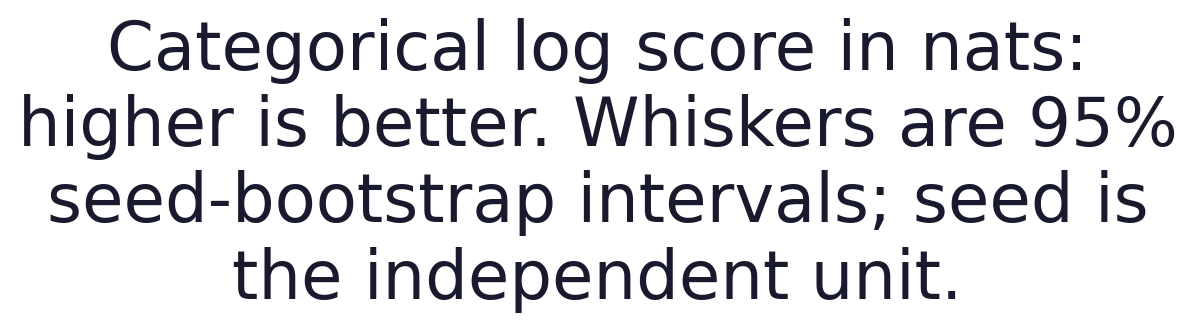
\includegraphics[keepaspectratio,width=0.98\linewidth,height=0.8\textheight,alt={Categorical log score in nats: higher is better. Whiskers are 95\% seed-bootstrap intervals; seed is the independent unit.}]{../figures/belief_quality.slide-score-key.png}
\refstepcounter{figure}\label{fig:belief-quality-slide-panel-7}
\end{figure}
\end{frame}

\begin{frame}{Proper scores and\ldots{} (part 12)}
\begin{figure}
\centering
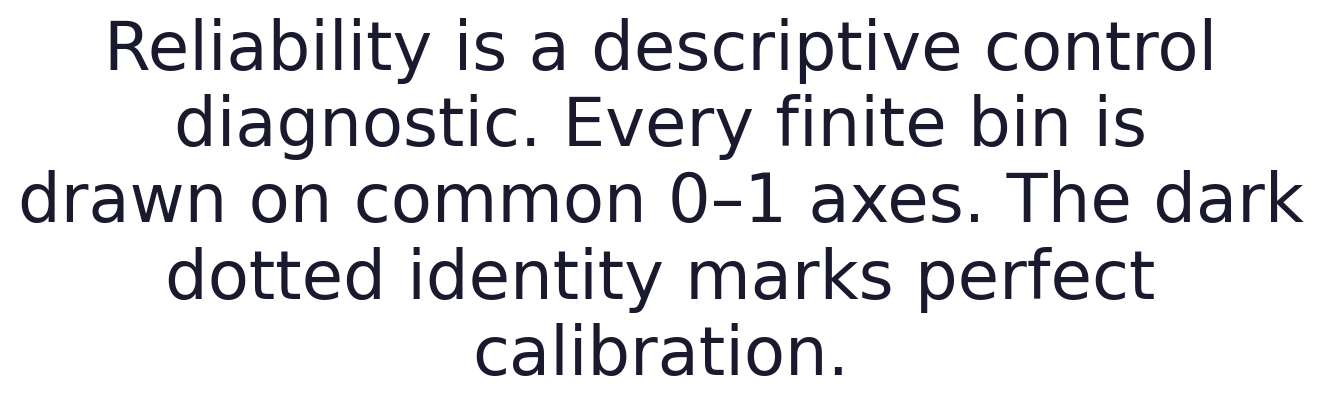
\includegraphics[keepaspectratio,width=0.98\linewidth,height=0.8\textheight,alt={Reliability is a descriptive control diagnostic. Every finite bin is drawn on common 0--1 axes. The dark dotted identity marks perfect calibration.}]{../figures/belief_quality.slide-reliability-key.png}
\refstepcounter{figure}\label{fig:belief-quality-slide-panel-8}
\end{figure}
\end{frame}

\begin{frame}{Proper scores and\ldots{} (part 13)}
\begin{figure}
\centering
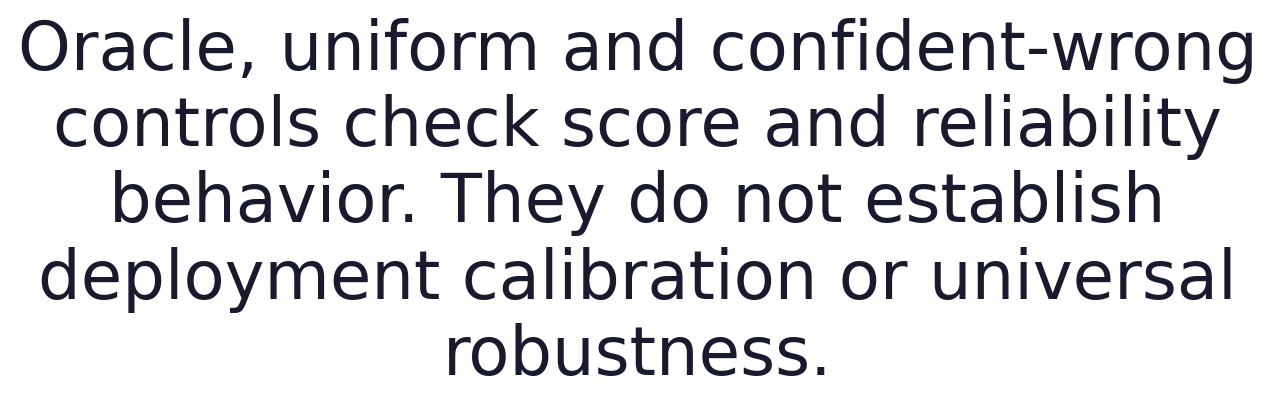
\includegraphics[keepaspectratio,width=0.98\linewidth,height=0.8\textheight,alt={Oracle, uniform and confident-wrong controls check score and reliability behavior. They do not establish deployment calibration or universal robustness.}]{../figures/belief_quality.slide-scope.png}
\refstepcounter{figure}\label{fig:belief-quality-slide-panel-9}
\end{figure}
\end{frame}

\begin{frame}[fragile]{Greedy multi-hypothesis model reduction beyond
the main BMR study}
\protect\phantomsection\label{sec:supp-greedy-bmr}
The single-step reduction of sec.~5.4 scores one
candidate reduced prior. \texttt{bayesian\_model\_reduction.py} adds
\texttt{greedy\_reduce}, which performs structure learning over a
\emph{family} of redundant states:
\end{frame}

\begin{frame}{Greedy multi-hypothesis\ldots{} (part 2)}
starting from the full prior, it scores pruning each not-yet-pruned
state against the current reduced prior, accepts the single prune with
the largest positive free-energy gain,

and repeats until no remaining prune improves model evidence.
\end{frame}

\begin{frame}{Greedy multi-hypothesis\ldots{} (part 3)}
Every accepted step has a strictly positive incremental \(\Delta F\), so
the cumulative evidence is monotone-increasing and the search recovers
the sparse generative model the data support --- a state with genuine
evidence yields \(\Delta F < 0\) when pruned and is kept.
\end{frame}

\begin{frame}{Greedy multi-hypothesis\ldots{} (part 4)}
This is the multi-state analogue of the configured BMR sign-control
result of sec.~7.4, and is verified directly in
the model-reduction tests.
\end{frame}

\end{document}
